% !TEX program = xelatex
\documentclass{VUMIFPSkursinis}
\usepackage{algorithmicx}
\usepackage{algorithm}
\usepackage{algpseudocode}
\usepackage{amsfonts}
\usepackage{amsmath}
\usepackage{bm}
\usepackage{caption}
\usepackage{color}
\usepackage{float}
\usepackage{graphicx}
\usepackage{listings}
\usepackage{subfig}
\usepackage{array}
\usepackage{wrapfig}

\usepackage[hidelinks]{hyperref}
\usepackage{multirow}
\usepackage{longtable}

\newcolumntype{L}[1]{>{\raggedright\let\newline\\\arraybackslash\hspace{0pt}}p{#1}}
\newcolumntype{C}[1]{>{\centering\let\newline\\\arraybackslash\hspace{0pt}}p{#1}}
\newcolumntype{R}[1]{>{\raggedleft\let\newline\\\arraybackslash\hspace{0pt}}p{#1}}

% Titulinio aprašas
\university{Vilniaus universitetas}
\faculty{Matematikos ir informatikos fakultetas}
\department{}
\papertype{Reikalavimų inžinerijos pirmas laboratorinis darbas - reikalavimų specifikacija}
\title{Epidemiologinės šalies situacijos sekimo sistema}
\titleineng{Epidemiologinė sistema}
\status{1 kurso PS magistrantūros studentai}
\author{Šarūnas Kazimieras Buteikis}
\secondauthor{Matas Savickis}
\thirdauthor{Rokas Ulickas}
\fourthauthor{Vytautas Krivickas}
\supervisor{dr. Audronė Lupeikienė}
\date{Vilnius – \the\year. Versija 1.0}

% Nustatymai
% \setmainfont{Palemonas} % Pakeisti teksto šriftą į Palemonas (turi būti įdiegtas sistemoje)
\bibliography{bibliografija}

\begin{document}

\maketitle

\sectionnonumnocontent{Santrauka}

Šiame dokumente pateikiama „Epidemiologinės šalies situacijos sekimo sistemos“ reikalavimų specifikacija: 
naudojantis Zachmano karkasu suformuluoti verslo, vartotojo, IS ir programinės įrangos reikalavimai. Komandą sudarė:
\begin{itemize}
	\item Šarūnas Kazimieras Buteikis (el. paštas \href{mailto:sarunas.buteikis@mif.stud.vu.lt}{sarunas.buteikis@mif.stud.vu.lt}) -- dokumento maketavimas, gramatikos taisymas, verslo, programų sistemų reikalavimai.
	\item Vytautas Krivickas (el. paštas \href{mailto:vytautas.krivickas@mif.stud.vu.lt}{vytautas.krivickas@mif.stud.vu.lt}) -- dokumento maketavimas, įžanga, verslo reikalavimai, naudotojo reikalavimai išvados.
	\item Matas Savickis (el. paštas \href{mailto:matas.savickis@mif.stud.vu.lt}{matas.savickis@mif.stud.vu.lt}) -- dokumento maketavimas, verslo reikalavimai, IS reikalavimai, programinės įrangos reikalavimai.
	\item Rokas Ulickas (el. paštas \href{mailto:rokas.ulickas@mif.stud.vu.lt}{rokas.ulickas@mif.stud.vu.lt}) -- verslo reikalavimai, IS reikalavimai, programinės įrangos reikalavimai.
\end{itemize}

\newpage

\tableofcontents

\section{Įžanga}
Šiame dokumente aprašoma „Epidemiologinės šalies situacijos sekimo sistema”, toliau - „epidemiologinė sistema” arba „sistema”.
Ši sistema skirta sekti epidemiologinei padėčiai šalyje: įvertinti viruso plitimo šalyje tendencijas,
efektyviai identifikuoti naujus viruso židinius, leisti specialistams atsekti susirgusiųjų
kontaktus registruojant užsikrėtusiųjų maršrutus ir potencialiuose rizikos židiniuose
besilankančius žmones, greitai informuoti kontaktavusiuosius su užsikrėtusiu žmogumi
apie privalomą saviizoliaciją, rinkti duomenis apie asmenis karantine.

\subsection{Pritaikymo sritis}
Ši sistema skirta naudoti sveikatos apsaugos sistemoje: sistema turėtų palengvinti
epidemiologų darbą ir leisti sekti viruso plitimą populiacijoje, imtis efektyvesnės
profilaktikos ir tirti naudojamų priemonių efektyvumą.

\subsection{Probleminė sritis}
Sistema siekiama išspręsti šias problemas:
\begin{itemize}
	\item Atskirų sveikatos įstaigų renkami susirgimų duomenys nėra apdorojami centralizuotai
	      arba tai daroma ne sistemingai, todėl epidemiologams sunku identifikuoti tikrąsias viruso
	      plitimo šalyje tendencijas, greitai identifikuoti potencialius židinius.
	\item Dėl žmogiškųjų resursų trūkumo dažnai tampa neįmanoma įspėti visų kontaktavusiųjų
	      su užsikrėtusiuoju asmenų - automatizavus šį procesą būtų galima įgyvendinti efektyvesnę
	      profilaktiką, užkardyti nevaldomą epidemijos plitimą.
	\item Šiuo metu nėra centralizuotos sistemos, leidžiančios registruoti potencialiuose
	      rizikos židiniuose (įvairiuose renginiuose, masinio susibūrimo vietose) besilankančius
	      asmenis, dabar egzistuojančios pavienės iniciatyvos neleidžia automatiškai atsekti reikšmingo kiekio susirgusiojo kontaktų - tenka pasikliauti pastarojo pateikta informacija.
	\item Nacionalinio sveikatos centro darbuotojai neturi galimybės automatiškai įspėti
	      atvykusiųjų iš pavojingų šalių asmenų apie privalomą saviizoliaciją: atlikus reikiamas
	      integracijas su muitinės sistemomis, ši sistema leistų automatizuoti ir šį procesą.
	\item Šiuo metu nėra galimybės automatizuoti saviizoliacijos reikalavimų laikymosi sekimo,
	      tad naujoji sistema leistų bent iš dalies automatizuoti šį procesą: reikalauti asmenis
	      saviizoliacijoje pateikti savo dabartinę vietą naudojantis išmaniajame telefone esančia
	      GPS sistema ar atsiųsti saviizoliaciją patvirtinančią nuotrauką.
\end{itemize}

\subsection{Naudotojai}
Šios sistemos naudotojų bazę sudaro trijų kategorijų naudotojai:
\begin{itemize}
	\item Epidemiologai - tai savo srities ekspertai, turintys aukštąjį išsilavinimą.
	      Naudotis sistema jiems pakaks mokykloje dėstomo informatikos kurso.
	\item LR esantys asmenys, dalyvaujantys riziką turinčiuose renginiuose, esantys saviizoliacijoje,
	      atvykę iš pavojingų šalių ar turėję sąlytį su sergančiaisiais - jiems taip pat pakaks
	      mokykloje dėstomo informatikos kurso.
	\item Duomenų analitikai - tam, jog galėtų efektyviai panaudoti sistemoje
	      esančius duomenis jiems reikalingas bakalauro ar aukštesnis iššsilavinimas
	      duomenų mokslo ar informatikos srityse.
\end{itemize}

\subsection{Darbo priežastys}
Darbe aprašoma sistema ypač aktuali rudenį prasidėjus antrajai korona viruso bangai. Tokia sistema padėtų 
valdyti viruso plitimą bei suteiktų epidemiologams vertingų įžvalgų.

\subsection{Šaltiniai}
\begin{enumerate}
	\item A. Čaplinskas, REIKALAVIMŲ INŽINERIJA, Vilnius 2010.
	\item A. Lupeikienė, Requirements Engineering paskaitų medžiaga, Vilnius 2020.
\end{enumerate}

\newpage

\section{Reikalavimų artefaktai} \label{sec:artefaktai}
Šiame skyriuje pateikiami gauti reikalavimų artefaktai, kuriant reikalavimų specifikaciją pagal Zachmano karkasą.
\begin{center}
\small
\begin{longtable}{|L{4cm}|L{4cm}|L{4cm}|L{4cm}|}
\caption{Verslo lygio reikalavimai: „Kodėl?", „Kaip?", „Ką?"}
\label{table:BusinessReq-WhyHowWhat}
		\\ \hline
		                                                 & Kodėl? (motyvacija) & \multicolumn{1}{c|}{Kaip? (veiklos)} & Ką? (apdorojami objektai)                                                                                                                                                                                                                                                                                                                                                                                                                                                                                                                                           \\ \hline
		Verslo reikalavimai  (verslo inžinieriaus požiūris)&
		\ref{sec:versloReqWhy} skyrelis&
		1.Galimybė valdyti duomenis apie žmones susirgusius virusu.
		2.Galimybė valdyti duomenis apie naujus ligos atvejus.
		3.Galimybė registruoti užsikrėtusių žmonių maršrutus.
		4.Galimybė perduoti statistiką suinteresuotoms asmenims.
		5.Galimybė valdyti pavojingų šalių sąrašą.
		6.Galimybė valdyti informaciją apie saviizoliacijos pažeidimus.
		7.Galimybė valdyti duomenis apie iš pavojingų šalių atvykstančius asmenis.
		8.Galimybė valdyti duomenis apie masinius renginius.
		9.Galimybė valdyti duomenis apie viešojo maitinimosi įstaigas.
		10.Galimybė valdyti duomenis apie asmens rizikos faktorius.
		11.Galimybė valdyti informaciją apie asmens saviizoliacijos patvirtinimą.
		12.Galimybė valdyti asmenų sveikatos informaciją &
		\textbf{Verslo objektai (esybės):} Privatus asmuo, Renginių organizatorius; Maitinimo / pasilinksminimo įstaigos atstovas; Karštosios linijos operatorius; NVSC departamento epidemiologas; Sveikatos apsaugos ministerija; Nacionalinis visuomenės sveikatos centras; Muitinė; Valstybė; E.\newline \textbf{Verslo objektai (procedūros):} Užsiregistruoti; Patvirtinti saviizoliaciją; Būti įspėtam apie riziką (galima kontaktą); Užregistruoti renginį; Užregistruoti įstaigą; Užregistruoti atvejį; Užregistruoti maršrutą; Pateikti pavojingų šalių sąrašą; Gauti epidemiologinę statistiką; Pateikti iš pavojingų šalių atvykusių žmonių sąrašą; Kontroliuoti saviizoliaciją \\ \hline
\end{longtable}

\begin{longtable}{|L{4cm}|L{4cm}|L{4cm}|L{4cm}|}

\caption{Verslo lygio reikalavimai: „Kas?", „Kur?", „Kada?"}
\label{table:BusinessReq-WhoWhereWhen}
\\ \hline
		                          & Kas? (funkciniai vienetai) & Kur? (vieta) & Kada? (laikas) \\ \hline
		\begin{tabular}[c]{@{}l@{}}Verslo reikalavimai \\ (verslo inžinieriaus \\ požiūris) \end{tabular} & \ref{sec:versloReqWho} skyrelis& \ref{sec:versloReqWhere} skyrelis              & \ref{sec:versloReqWhen} skyrelis                \\ \hline
\end{longtable}

\begin{longtable}{|L{4cm}|L{4cm}|L{4cm}|L{4cm}|}
\caption{Vartotojo lygio reikalavimai: „Kodėl?", „Kaip?", „Ką?"}
\label{table:UserReg-WhyHowWhat}
\\ \hline
		                                                & Kodėl? (motyvacija) & \multicolumn{1}{c|}{Kaip? (veiklos)} & Ką? (apdorojami objektai) \\ \hline
		Vartotojo reikalavimai (dalykinės srities specialisto požiūris)
		& \ref{sec:vartotojoReqWhy} skyrelis & \ref{sec:vartotojoReqHow} skyrelis & \ref{sec:vartotojoReqWhat} skyrelis                               \\ \hline

\end{longtable}

\begin{longtable}{|L{4cm}|L{4cm}|L{4cm}|L{4cm}|}

\caption{Vartotojo lygio reikalavimai: „Kas?", „Kur?", „Kada?"}
\label{table:UserReq-WhoWhereWhen} \\ \hline
		                                                                                                                                                    & Kas? (funkciniai vienetai) & \multicolumn{1}{c|}{Kur? (vieta)} & Kada? (laikas) \\ \hline
		Vartotojo reikalavimai (dalykinės srities specialisto požiūris
		& \ref{sec:vartotojoReqWho} skyrelis & \ref{sec:vartotojoReqWhere} skyrelis & \ref{sec:vartotojoReqWhen} skyrelis                                                                                                                                        \\ \hline
	
\end{longtable}

\begin{longtable}{|L{4cm}|L{4cm}|L{4cm}|L{4cm}|}

\caption{Informacinių sistemų lygio reikalavimai: „Kodėl?", „Kaip?", „Ką?"}
\label{table:ISReq-WhyHowWhat} \\ \hline
		                          & Kodėl? (motyvacija) & \multicolumn{1}{c|}{Kaip? (veiklos)} & Ką? (apdorojami objektai) \\ \hline
		IS reikalavimai (IS inžinieriaus požiūris)
		&\ref{sec:ISReqWhy} skyrelis  &\ref{sec:ISReqHow} skyrelis& \ref{sec:ISReqWhat} skyrelis \\ \hline
	
\end{longtable}

\begin{longtable}{|L{4cm}|L{4cm}|L{4cm}|L{4cm}|}

\caption{Informacinių sistemų lygio reikalavimai: „Kas?", „Kur?", „Kada?"}
\label{table:ISReq-WhoWhereWhen} \\ \hline
		                          & Kas? (funkciniai vienetai) & \multicolumn{1}{c|}{Kur? (vieta)} & Kada? (laikas) \\ \hline
		IS reikalavimai (IS inžinieriaus  požiūris)& \ref{sec:ISReqWho} skyrelis                           &  \ref{sec:ISReqWhere} skyrelis                                 & \ref{sec:ISReqWhen} skyrelis               \\ \hline

\end{longtable}

\newpage
\begin{longtable}{|L{4cm}|L{4cm}|L{4cm}|L{4cm}|}

\caption{Programų Sistemų lygio reikalavimai: „Kodėl?", „Kaip?", „Ką?"}
\label{table:PSReq-WhyHowWhat} \\ \hline
		                                                                                                             & Kodėl? (vizija ir suvaržymai) & Kaip? (sistemos panaudojimo atvejai ir kokybė) & Ką(duomenys ir jų sauga) \\ \hline
		Programos reikalavimai (Kiekvienai sistemai)                                                                                   &
		\ref{sec:PSReqWhy} skyrelis &

		Programų sistema įgyvendina visus funkcinius ir nefunkcinius reikalavimus atsižvelgdama ekonominius ir politinius reikalavimus iškeltus suinteresuotų šalių 
		stengiantis nesumažinti sistemos kokybės.
		Turi būti pasiektas nurodytas patikimumas bei diegimo ir palaikymo procedūros ateities sistemos vystytojas.

		                                                                                                             &
		Sistemoje yra saugomi privačių asmenų asmeninai duomenys bei su jų sveikatos būkle susiję duomenys.
		Sistema turi užtikrinti, kad neautorizuoti ir blogi aktoriai negalėtų pasiekti privačių asmenų duomenų.
		Duomenys turi būti apsaugoti ne tik nuo išorinių blogų aktorių, bet ir nuo sistemos kūrėjų ir palaikytojų klaidų,
		duomenis apsaugant nuo atsitiktinio jų ištrynimo ar modifikavimo.
		Visas disponavimas duomenimis turi atitikti Lietuvos ir Europos įstatymus.                                                                                                                                               \\ \hline

\end{longtable}


\begin{longtable}{|L{4cm}|L{4cm}|L{4cm}|L{4cm}|}

\caption{Programų Sistemų lygio reikalavimai: „Kas?", „Kur?", „Kada?"}
\label{table:PSReq-WhoWhereWhen} \\ \hline
		                           & Kas? (vartotojo sąsajos, prieinamumo ir ergonomikos reikalavimai) & Kur? (sistemos platformos reikalavimai) & Kada? (laiko suvaržymai aplikacijos panaudojimo atvejuose) \\ \hline
		Programos reikalavimai (Kiekvienai sistemai) &

		Sistema turi būti pritaikyta naudotis vartotojams su regos sutrikimais.
		Turi būti galimybė keisti vartotojo sąsajos spalvų gama labiau pritaikytą daltonikams.
		Sistema taip turi suteikti galimybė padidinti vartotojo sąsajos tekstą ir elementų dydį bei spalvą
		padedant žmonėms su silpnu regėjimu.
		Sistema turi turėti apmokymo programą naujiems vartotojams su įvairiais kompiuterinio raštingumo lygiais,
		tačiau daroma prielaida, kad vartotojas turi bazinius kompiuterinio raštingumo įgūdžius.
		Patyrusiems vartotojas sistema turi suteikti greitojo vedimo ir sisteminių klaviatūros trumpinių galimybę taip pagreitinant patyrusio vartotojo darbą.
		Sistema turi išsijungti po 30 minučių neaktyvumo.
		Sėkmingai atlikta užduotis sistemoje turi būti identifikuojama garsiniu signalu.
		Visa sistema turi būti sukurta laikanti žmogaus ir kompiuterio sąveikos euristikų.

		                           &

		Sistema veiks mikroservisų architektūros principu naudojant AWS debesijos sistema.
		Papildomi sisteminiai resursai bus padidinami ir sumažinami pagal sistemos apkrovas.
		Sistemos vartotojai sistemą pasiekti galės naudodamiesi vidutinio galingumo stacionariu kompiuteriu Windows 10 aplinkoje.

		                           &

		Sistema efektyviai turi veikti 24h per parą.
		Didžiausia apkrova sistemai bus darbo valandomis kai yra paskelbiama nauji viruso atvejai.
		Sistemoje svarbu užtikrinti duomenų integralumą, kad visi siunčiami ir gaunami duomenys galiausiai būtų išsaugomi.
		Sistema turi palaikyti didelį įrašų kiekį ir jų siuntinėjimą tiek siunčiant informacija kitiems sistemos aktoriams tiek ir gaunant žinutes iš tų pačiu aktorių.
		Duomenų integralumas turi būti išsprendžiamas per vieną minutę.
		Viena transakcija negali trukti ilgiau negu 0,1 sekundės.

		\\ \hline

\end{longtable}
\end{center}

\section{Verslo reikalavimai}\label{sec:versloReq}
Šiame skyriuje nagrinėjami verslo reikalavimai Epidemiologinės šalies situacijos sekimo sistemai.
\subsection{Kodėl?}\label{sec:versloReqWhy}

\begin{figure}[H]
	\centering
	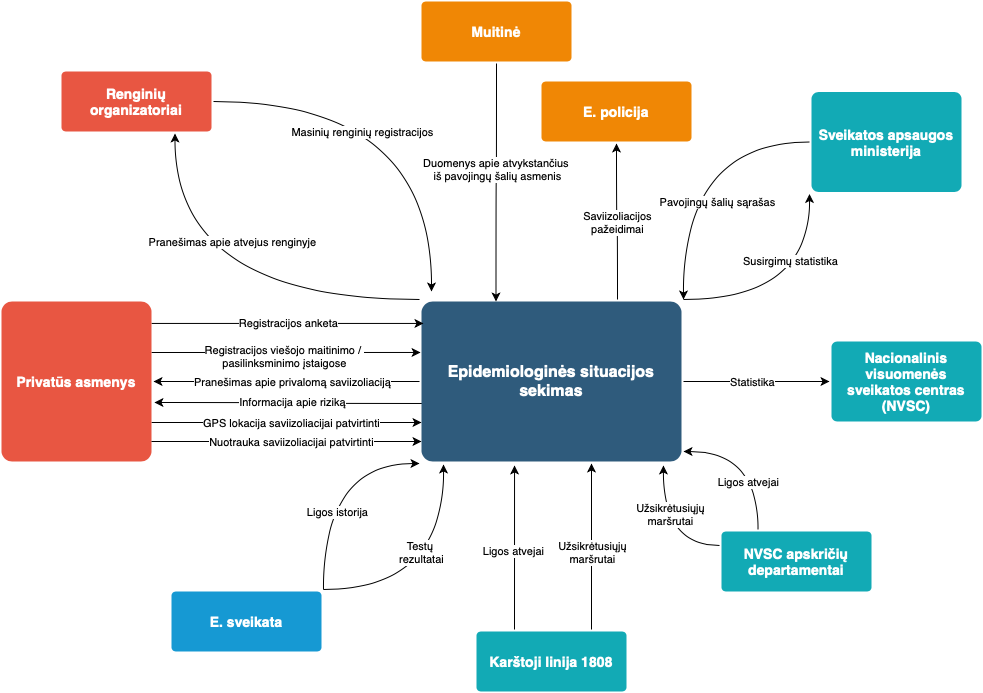
\includegraphics[scale=0.5]{img/context_diagram.png}
	\caption{Konteksto diagrama}
	\label{img:context_diagram}
\end{figure}

\subsubsection{Išorinė verslo analizė}\label{sec:versloReqWhyAnalysis}

\begin{figure}[H]
	\centering
	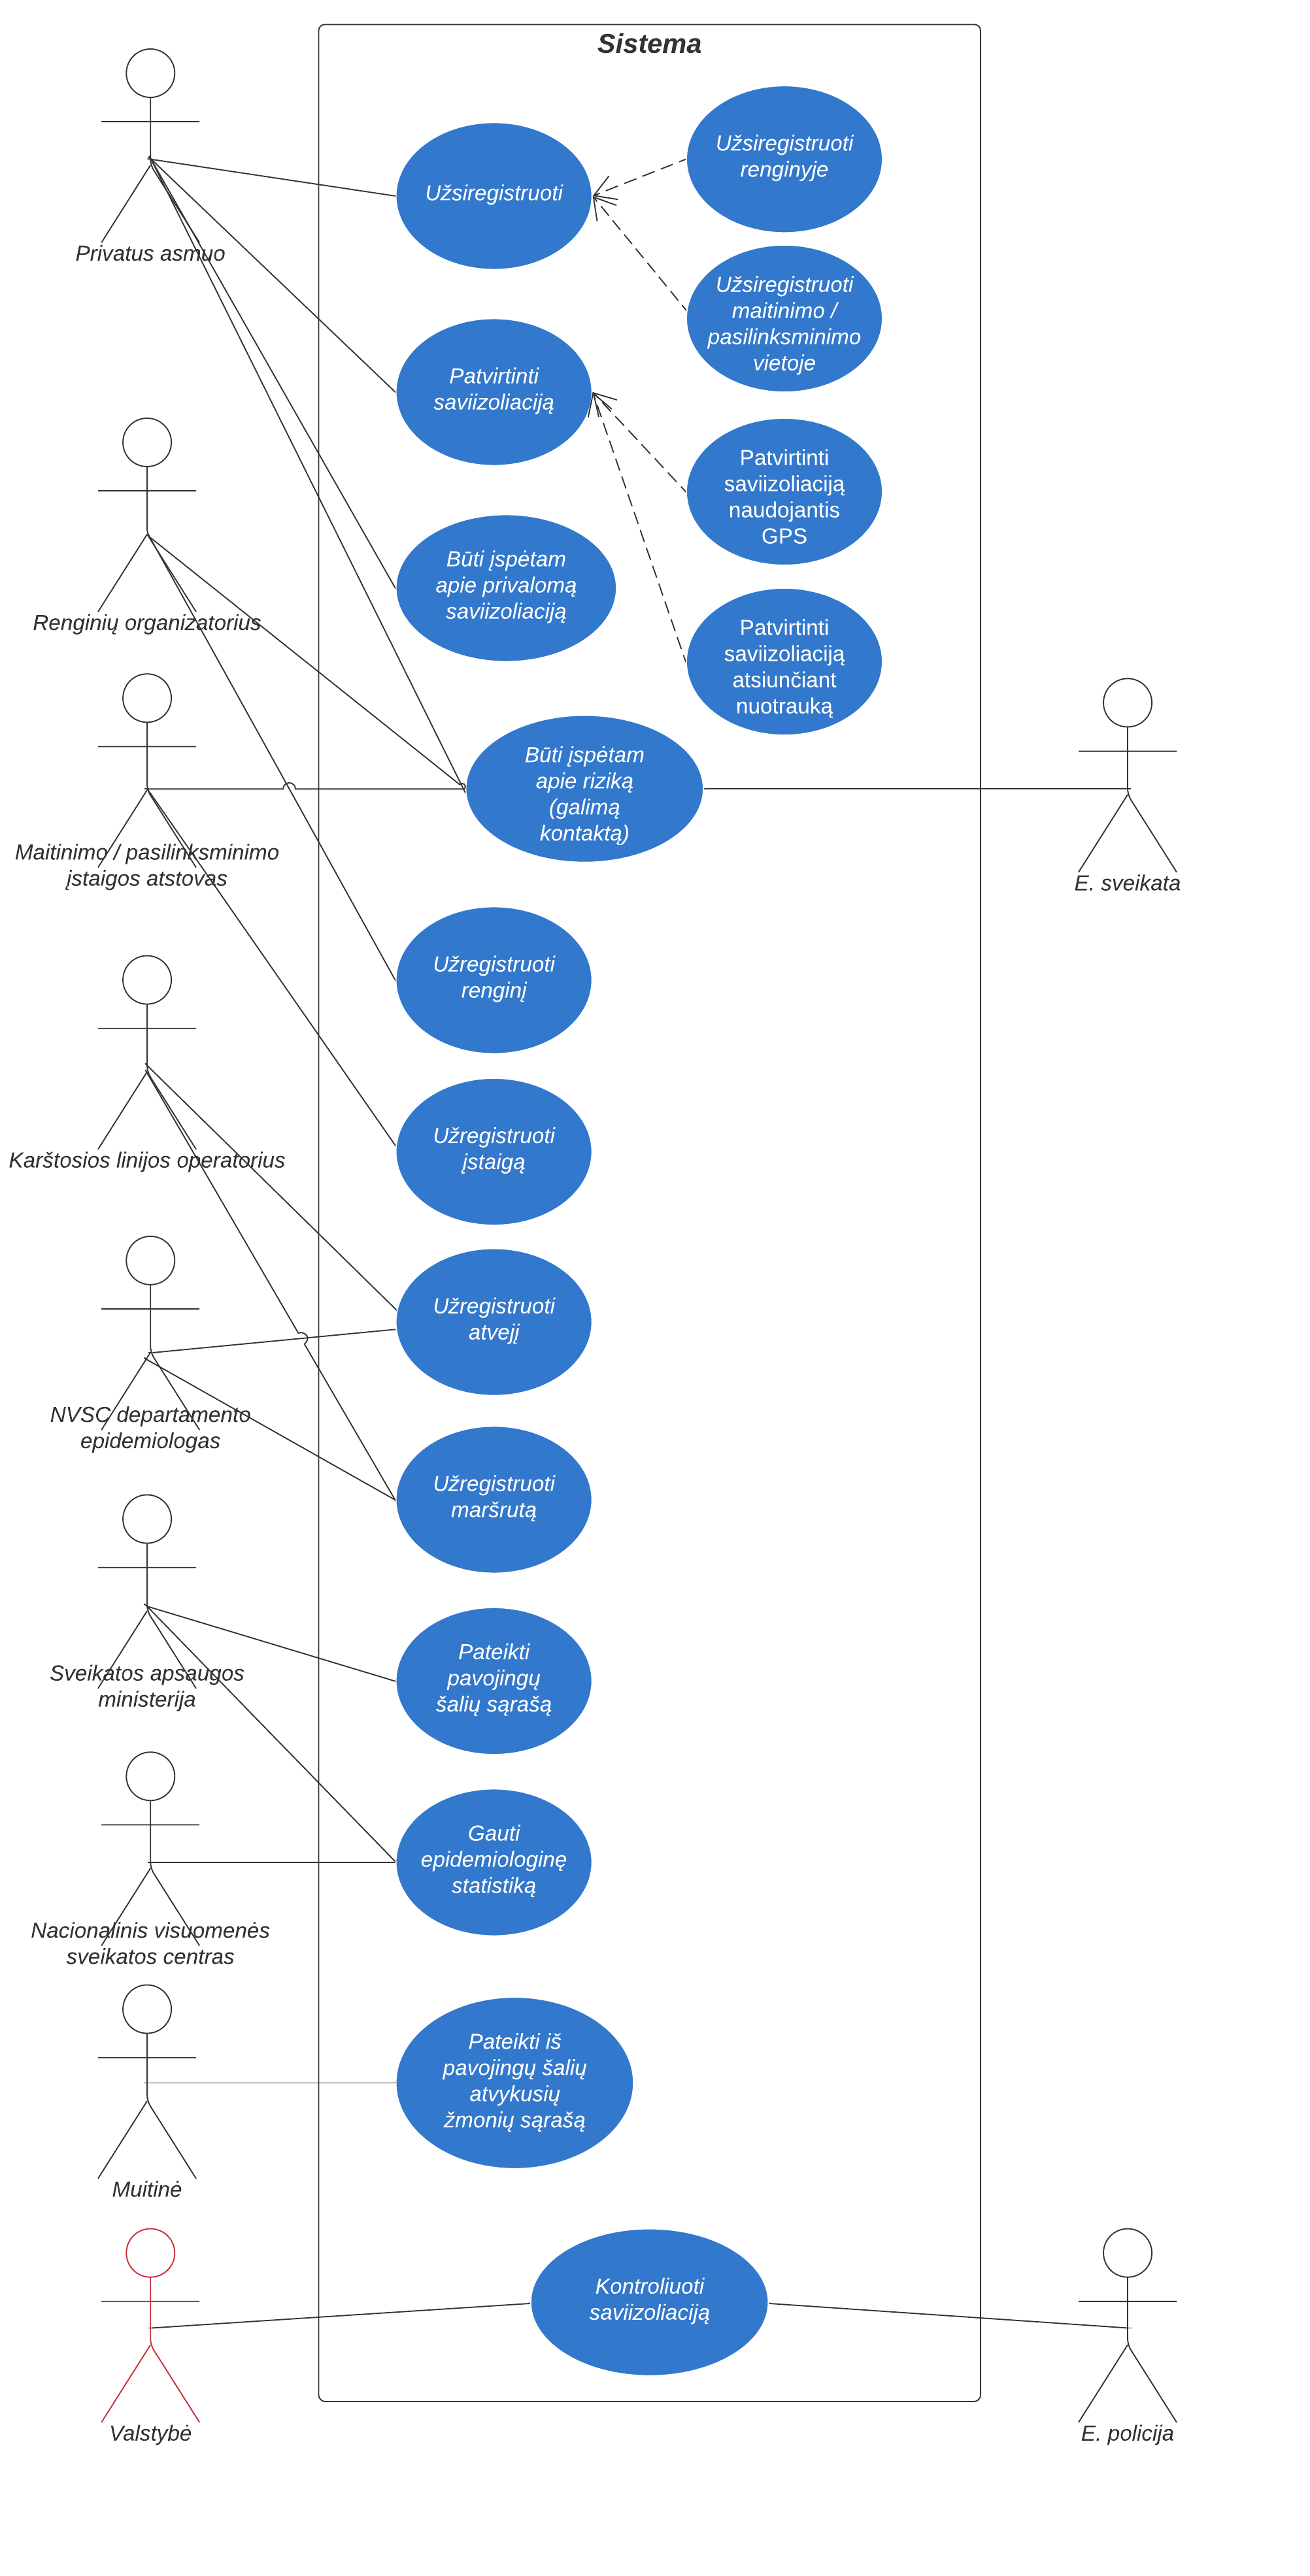
\includegraphics[scale=0.6]{img/use_case_diagram_business.png}
	\caption{Verslo užduočių diagrama}
	\label{img:use_case_diagram}
\end{figure}
\newpage
\subsubsection{Įvestys}\label{sec:versloReqWhyInput}

\begin{center}
\begin{longtable}{|L{0.5cm}|L{4cm}|L{3cm}|}

\caption{Įvestys}
\label{table:input} \\ \hline
			
			\textbf{Nr.}        & \textbf{Įvestis}  & \multicolumn{1}{c|}{\textbf{Įvertinimo parametrai}} \\ \hline
			\multirow{2}{*}{I1} & \multirow{2}{*}{\parbox{4cm}{Registracijos didesnės rizikos renginiuose}} & Kiekis \\ \cline{3-3}
			                    &                                                             & Korektiškumas \\ \hline
			I2                  & Registracijos viešojo maitinimo įstaigose                  &                \\ \hline
			I3                  & Informacija apie keliones iš rizikos šalių                  &               \\ \hline
			I4                  & Pavojingų šalių sąrašas                                     &               \\ \hline
			I5                  & Asmenų ligos istorijos                                      &               \\ \hline
			I6                  & Testų rezultatai                                            &               \\ \hline
			I7                  & Saviizoliaciją patvirtinantys vietos nustatymo duomenys     &               \\ \hline
			I8                  & Saviizoliaciją patvirtinanti nuotrauką                      &               \\ \hline
			I9                  & Atvykusių iš pavojingų šalių žmonių sąrašas                 &               \\ \hline
			I10                 & Masinių renginių registracijos                              &               \\ \hline
			I11                 & Užsikrėtusiųjų maršrutai                                    &               \\ \hline
			I12                 & Pranešimai apie įtariamus atvejus                           &               \\ \hline
		%
	
\end{longtable}
\end{center}
\subsubsection{Išvestys}\label{sec:versloReqWhyOutput}

\begin{center}
\begin{longtable}{|L{0.5cm}|L{4cm}|L{3cm}|}

\caption{Išvestys}
\label{table:output} \\ \hline
			
			\textbf{Nr} & \textbf{Išvestis}                          & Įvertinimo parametrai \\ \hline
			\textbf{O1} & Statistika                                 &                       \\ \hline
			\textbf{O2} & Pranešimas apie priverstinę saviizoliaciją &                       \\ \hline
			\textbf{O3} & Pranešimas apie saviizoliacijos pažeidimą  &                       \\ \hline
			\textbf{O4} & Pranešimas apie riziką                     &                       \\ \hline
			\textbf{O5} & Pranešimas renginių org. apie atvejus      &                       \\ \hline
			\textbf{O6} &                                            &                       \\ \hline
			\textbf{O7} &                                            &                       \\ \hline
			\textbf{O8} &                                            &                       \\ \hline
			\textbf{O9} &                                            &                       \\ \hline
\end{longtable}
\end{center}

\subsubsection{Reguliacija}\label{sec:versloReqRegulation}
Sistemoje renkamų bei saugomų duomenų tvarkymą reglamentuoja Lietuvos Respublikos asmens duomenų teisinės apsaugos įstatymas,
Bendrasis duomenų apsaugos reglamentas. Saviizoliacijos tvarką bei organizatorių prievolę registruoti renginių dalyvius nustato
LR vyriausybės nutarimas dėl valstybės lygio ekstremalios situacijos paskelbimo. Atsakomybę už saviizoliacijos pažeidimus
apibrėžia baudžiamasis kodeksas.

\subsubsection{Įvaizdis}\label{sec:versloReqWhyAssessment}
Apibendrinant galima išskirti dvi grupes, vertinančias sistemos įvaizdį: specialistus, besinaudosiančius sistema
bei visuomenę. Abi grupės sistemos įvaizdį vertins visų pirma patikimumo aspektu: ar sistema veikia be trikdžių,
nepažeidžiamas duomenų saugumas. Specialistai taip pat įvertins sistemos efektyvumą -- kaip patogu atlikti reikiamas
užduotis bei greitį -- kaip greitai sistema veikia. Neigiamą sistemos įvaizdį visuomenėje galėtų lemti jautrių duomenų,
renkamų sistemoje, kiekis bei automatinė saviizoliacijos pažeidimų fiksavimo funkcija.

\begin{center}
\begin{longtable}{|L{0.7cm}|L{4cm}|L{3cm}|L{3cm}|L{3cm}|}

\caption{Grupės, vertinančios sistemos įvaizdį}
\label{table:assessment} \\ \hline
			\textbf{Nr}                   & \textbf{Grupė}                 & Įvertinimo parametrai & Kiekybiniai matai               & Kokybiniai matai                                                                                      \\ \hline
			\textbf{IM1}                  & Visuomenė                      & Patikimumas           &                                 & Pranešimai žiniasklaidoje ar soc. tinkluose apie prastą (klaidingą, lėtą, nepatogų) sistemos veikimą. \\ \hline
			\multirow{2}{*}{\textbf{IM2}} & \multirow{2}{*}{Profesionalai} & Patikimumas           & Sistemos pasiekiamumas (uptime) & Trikdžiai ar klaidos naudojantis sistema.                                                             \\ \cline{3-5}
			                              &                                & Patogumas             & Užduočių atlikimo greitis       & Naudotojo patirtis                                                                                    \\ \hline

\end{longtable}
\end{center}

\subsubsection{Vidinė verslo analizė}\label{sec:versloReqWhyInternalAnalysis}

\subsubsection{Vizija}\label{sec:versloReqWhyVision}
Tapti pagrindiniu viruso plitimo visuomenėje valdymo įrankiu specialistams.

\subsubsection{Misija}\label{sec:versloReqWhyMission}
Su viruso plitimu susijusių duomenų agregavimas, leidžiantis sekti jo plitimą, pateikti rekomendacijas,
įspėti visus rizikoje atsidūrusius asmenis, bei kontroliuoti saviizoliacijos laikymąsį.

\subsubsection{SWOT analizė}\label{sec:versloReqWhySWOT}

\begin{figure}[H]
	\centering
	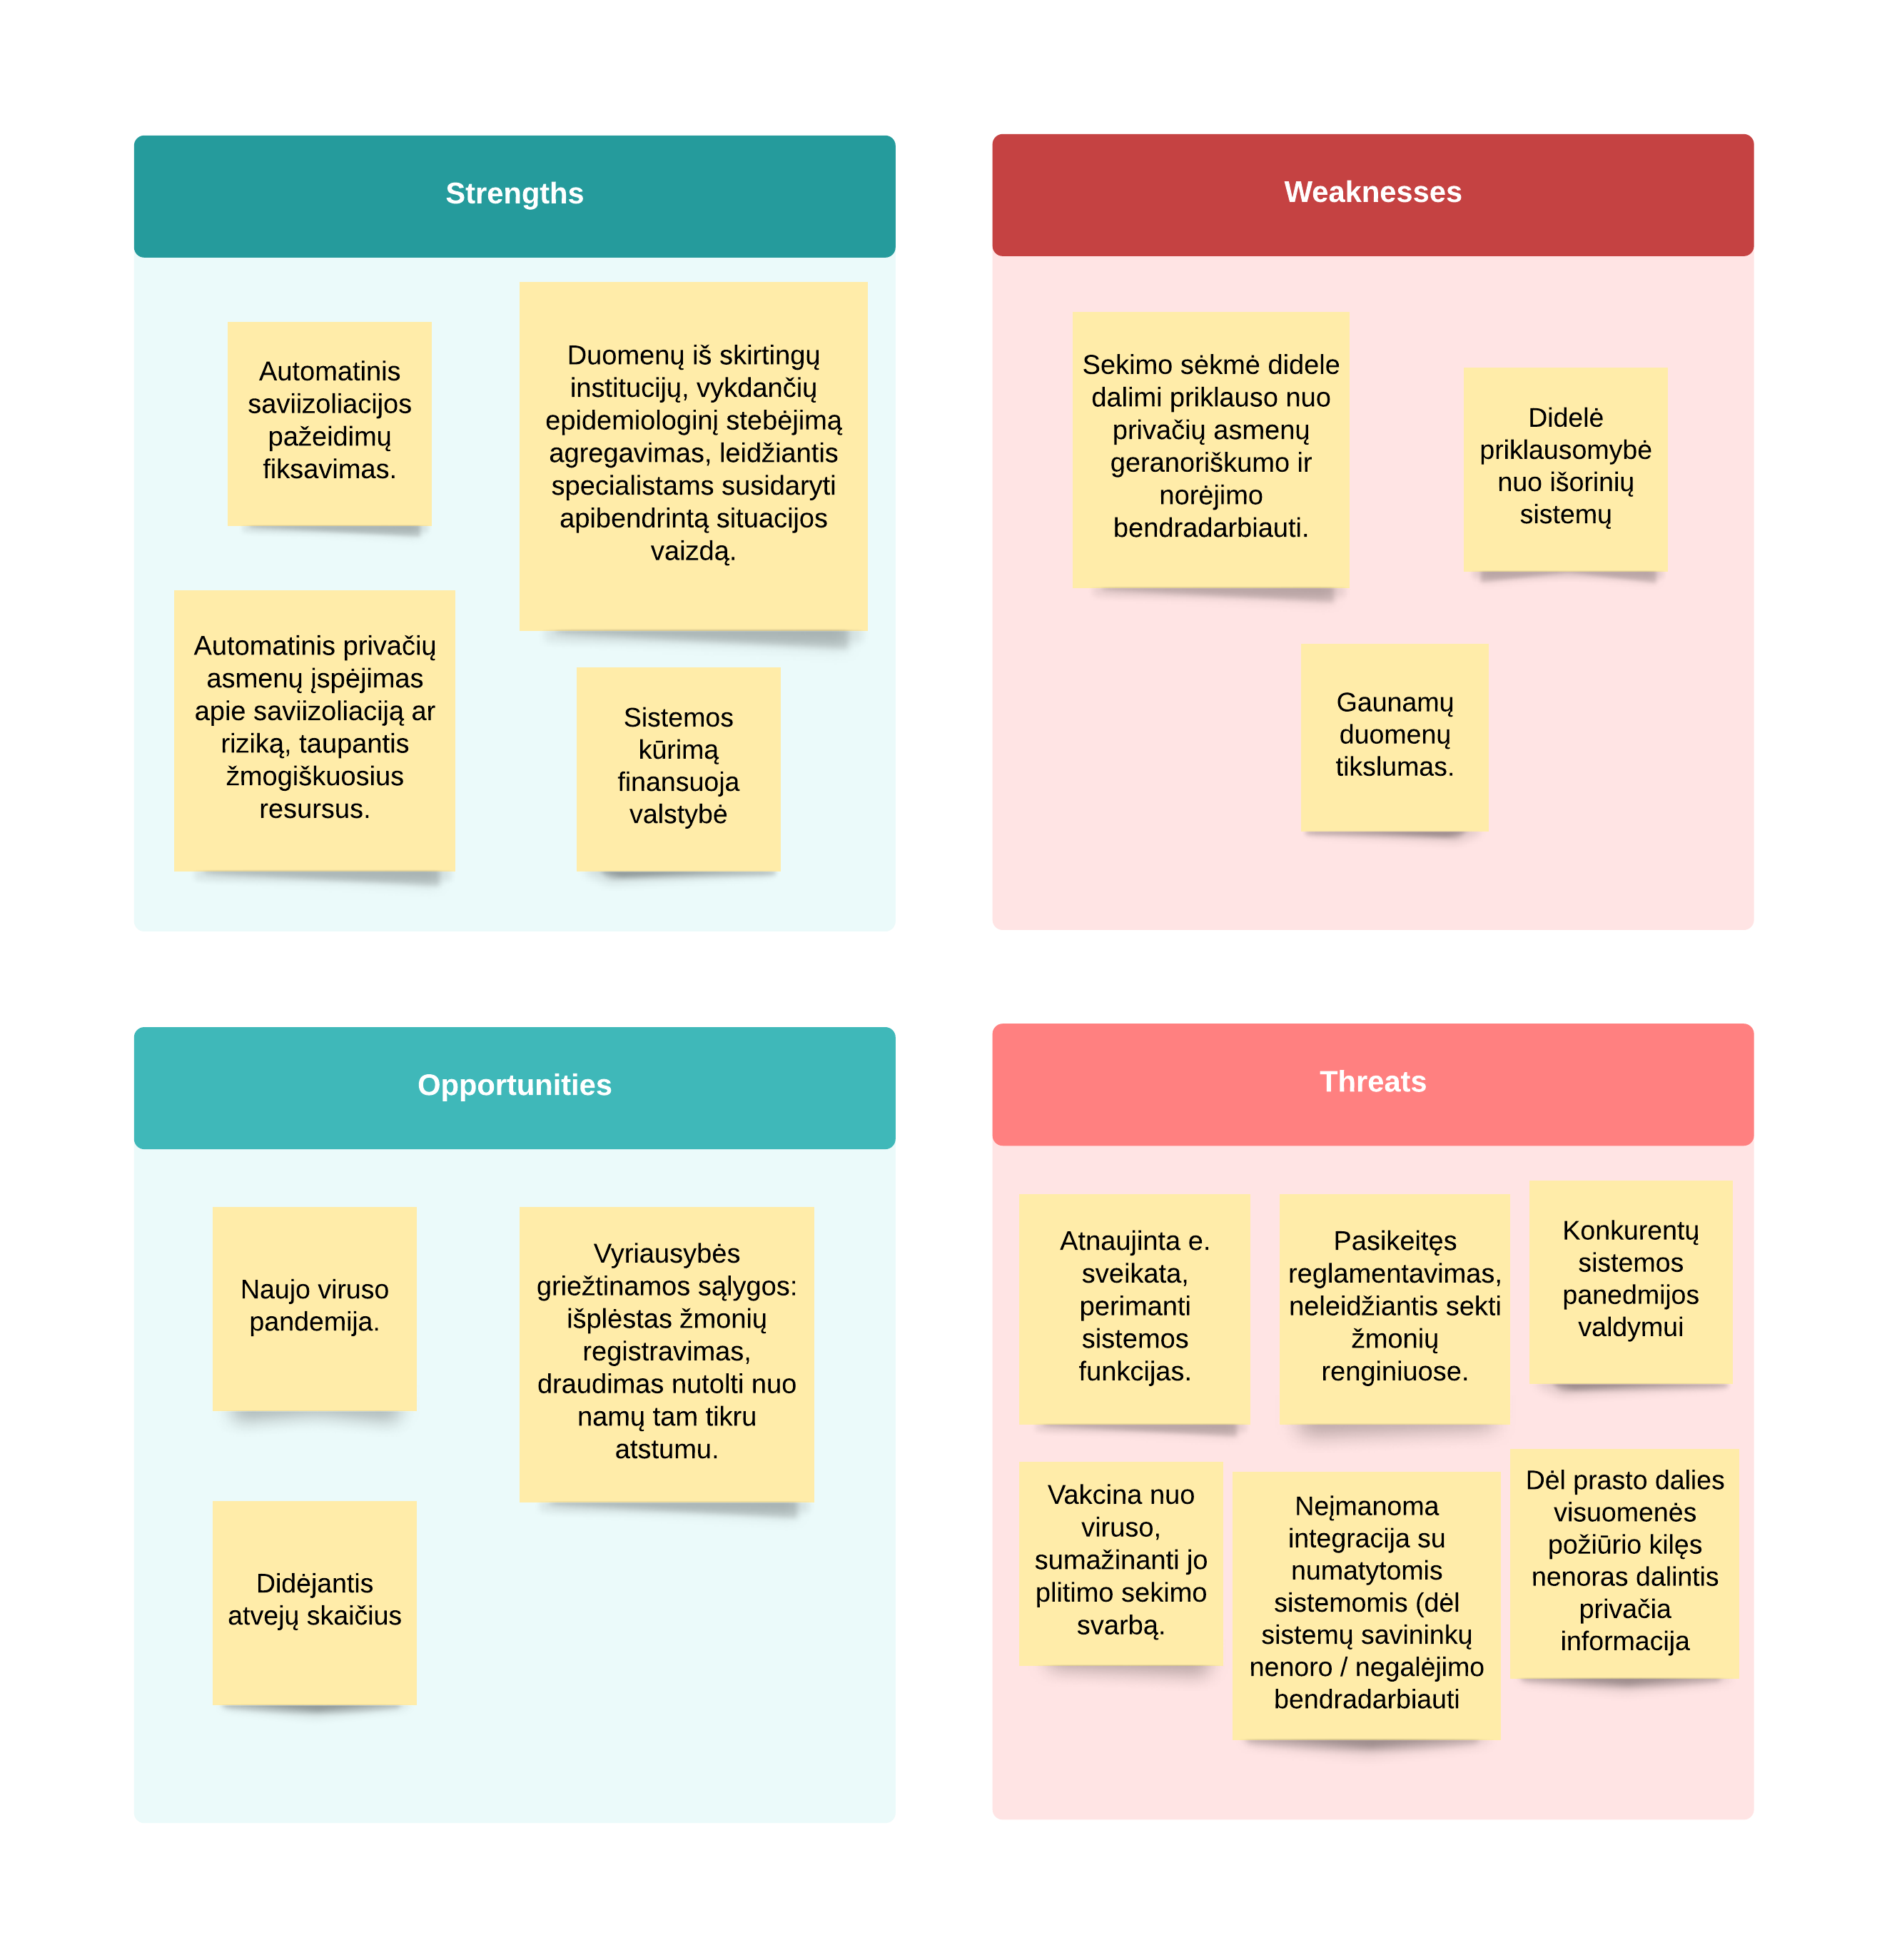
\includegraphics[scale=0.7]{img/SWOT.png}
	\caption{SWOT diagrama}
	\label{img:swot_diagram}
\end{figure}

\subsubsection{Siūloma verslo strategija}\label{sec:versloReqWhyStrategy}
Atsižvelgus į SWOT analizę, nuspręsta tolimesnę sistemos specifikaciją orientuoti pagal stiprybes: automatinį saviizoliacijos pažeidimų fiksavimą, duomenų agregavimą iš skirtingų institucijų, automatinį privačių asmenų įspėjimą apie saviizoliaciją ar riziką, sistemos kūrimą finansuoja valstybė.
\subsubsection{Tikslų medis}\label{sec:versloReqWhyObjTree}

\begin{enumerate}
	\item Tapti išsamiausiu duomenų apie viruso plitimą visuomenėje šaltiniu epidemiologams
	      \begin{enumerate}
		      \item Sukurti centralizuotą duomenų apie susirgimus registrą.
		      \item Sukurti centralizuotą duomenų apie maitinimo / pasilinksminimo įstaigų ir renginių lankytojus registrą.
	      \end{enumerate}
	\item Atlikti efektyvesnę viruso plitimo prevenciją
	      \begin{enumerate}
		      \item Įspėti privačius asmenis apie riziką.
		      \item Įspėti organizatorius apie atvejus renginiuose / įstaigose.
	      \end{enumerate}
	\item Užtikrinti platesnį saviizoliacijos laikymąsi.
	      \begin{enumerate}
		      \item Įspėti visus asmenims apie privalomą saviizoliaciją.
		            \begin{enumerate}
			            \item Identifikuoti asmenis, kuriems reikalinga saviizoliacija.
		            \end{enumerate}
		      \item Tikrinti saviizoliacijos laikymąsi.
		            \begin{enumerate}
			            \item Tikrinti asmens buvimo vietą.
		            \end{enumerate}
		      \item Pranešti apie pažeidimus policijai.
	      \end{enumerate}
\end{enumerate}

\subsection{Kaip?}\label{sec:versloReqHow}
\begin{enumerate}
	\item{Galimybė valdyti duomenis apie žmones susirgusius virusu.}
	\item{Galimybė valdyti duomenis apie naujus ligos atvejus.}
	      \begin{enumerate}
		      \item{Galimybė gauti duomenis apie naujus viruso atvejus iš „Karštoji linija 1808".}
		      \item{Galimybė gauti duomenis apie naujus viruso atvejus iš „NVSC apskričių departamentai".}
	      \end{enumerate}
	\item{Galimybė registruoti užsikrėtusių žmonių maršrutus.}
	      \begin{enumerate}
		      \item{Galimybė gauti duomenis apie užsikrėtusių žmonių maršrutus iš „Karštoji linija 1808"}
		            \begin{enumerate}
			            \item{Galimybė gauti žmogaus asmeninius duomenis, jų buvimo vietas per pastarąsias 21d. iš „Karštoji linija 1808" }
		            \end{enumerate}
		      \item{Galimybė gauti duomenis apie užsikrėtusių žmonių maršrutus iš „NVSC apskričių departamentai"}
		            \begin{enumerate}
			            \item{Galimybė gauti žmogaus asmeninius duomenis, jų buvimo vietas per pastarąsias 21d. iš „NVSC apskričių departamentai" }
		            \end{enumerate}
	      \end{enumerate}
	\item{Galimybė perduoti statistiką suinteresuotoms asmenims.}
	      \begin{enumerate}
		      \item{Galimybė pateikti statistinius duomenis „Nacionalinis visuomenės sveikatos centras"}
		      \item{Galimybė pateikti statistinius duomenis apie susirgusiu, pasveikusius asmenis ir atliktų testų statistiką.}
		      \item{Galimybė pateikti statistinius duomenis „Sveikatos apsaugos ministerija"}
		      \item{Galimybė pateikti statistinius duomenis apie susirgusiu, pasveikusius asmenis ir atliktų testų statistiką.}
	      \end{enumerate}
	\item{Galimybė valdyti pavojingų šalių sąrašą.}
	      \begin{enumerate}
		      \item{Galimybė gauti pavojingų šalių sąrašą iš „Sveikatos apsaugos ministerija"}
	      \end{enumerate}
	\item{Galimybė valdyti informaciją apie saviizoliacijos pažeidimus.}
	      \begin{enumerate}
		      \item{Galimybė pranešti apie saviizoliacijos pažeidimus „E. policja"}
		            \begin{enumerate}
			            \item{Galimybė perduoti „E. policija" susirgusio žmogaus įvykių sekimo žurnalą apie jo būseną per pastąrasias 21 dienas.}
		            \end{enumerate}
	      \end{enumerate}
	\item{Galimybė valdyti duomenis apie iš pavojingų šalių atvykstančius asmenis.}
	      \begin{enumerate}
		      \item{Galimybė gauti apie iš pavojingų šalių atvykstančius asmenis iš „Muitinė".}
	      \end{enumerate}
	\item{Galimybė valdyti duomenis apie masinius renginius.}
	      \begin{enumerate}
		      \item{Galimybė gauti duomenis apie masinius renginius iš ..Renginių organizatoriai"}
		            \begin{enumerate}
			            \item{Gauti žmonių dalyvaujančių renginyje skaičiu, dalyvių asmeninę inforaciją ir renginio vietos informaciją}
		            \end{enumerate}
		      \item{Gailmybė siųsti duomenis „Renginių organizatoriai" apie pavojingus asmenis.}
	      \end{enumerate}
	\item{Galimybė valdyti duomenis apie viešojo maitinimosi įstaigas.}
	      \begin{enumerate}
		      \item{Galimybė asmenims registruoti informaciją apie apsilankymus maitinimo įstaigose.}
		      \item{Galimybė pranešti maitinimo įstaigoms apie pavojingus asmenis.}
	      \end{enumerate}
	\item{Galimybė valdyti duomenis apie asmens rizikos faktorius.}
	      \begin{enumerate}
		      \item{Galimybė asmenims pranešti apie jų rizikos faktorius.}
		      \item{Galimybė asmenis informuoti apie saviizoliaciją.}
	      \end{enumerate}
	\item{Galimybė valdyti informaciją apie asmens saviizoliacijos patvirtinimą.}
	      \begin{enumerate}
		      \item{Galimybė sekti asmenis saviizoliacijos būseną.}
	      \end{enumerate}
	\item{Galimybė valdyti asmenų sveikatos informaciją}
	      \begin{enumerate}
		      \item{Galimybė gauti asmenų ligos istoriją iš „E. sveikata".}
		      \item{Galimybė gauti asmenų viruso testo rezultatus iš „E. sveikata".}
	      \end{enumerate}
\end{enumerate}

\subsection{Ką?}\label{sec:versloReqWhat}

Verslo objektai (esybės):
\begin{itemize}
	\item Privatus asmuo - Lietuvos Respublikoje gyvenantis fizinis asmuo.
	\item Renginių organizatorius - juridinis asmuo, kuris organizuoja renginius Lietuvos Respublikoje.
	\item Maitinimo/pasilinksminimo įstaigos atstovas - juridinis asmuo, atstovaujantis maitinimo/pasilinksminimo įstaigą.
	\item Karštosios linijos operatorius - verslo objektas, atitinkantis karštosios linijos operatorių tikrame pasaulyje.
	\item NVSC departamento epidemiologas - Juridinis asmuo, kuris užima NSVC departamento epidemiologo pareigas.
	\item Sveikatos apsaugos ministerija - verslo objektas, atitinkantis atitinkantis sveikatos apsaugos ministeriją tikrame pasaulyje.
	\item Nacionalinis visuomenės sveikatos centras - verslo objektas, atitinkantis nacionalinį visuomenės sveikatos centrą tikrame pasaulyje.
	\item Muitinė - verslo objektas, atitinkantis nacionalinį visuomenės sveikatos centrą tikrame pasaulyje.
	\item Valstybė - verslo objektas, atitinkantis Lietuvos Respublikos valstybę tikrame pasaulyje.
	\item E. policija - verslo objektas, atitinkantis elektroninės policijos sistemą tikrame pasaulyje.
\end{itemize}

\noindent Verslo objektai (procedūros):
\begin{itemize}
	\item Užsiregistruoti - privatus asmuo užsiregistruoja renginyje arba maitinimo/pasilinksminimo vietoje
	\item Patvirtinti izoliaciją - privatus asmuo patvirtina saviizoliaciją naudojantis GPS ir nusiunčiant jo koordinates arba atsiunčiant nuotrauką
	\item Būti įspėtam apie privalomą saviizoliaciją - privatus asmuo yra įspėjamas apie privalomą saviizoliaciją nurodytam laikui.
	\item Būti įspėtam apie riziką (galimą kontaktą) - privatus asmuo, renginių organizatorius arba maitinimo/pasilinksminimo įstaigos atstovas yra įspėjamas apie galima kontaktą su privačiu asmeniu, kuris galėjo sirgti viruso liga.
	\item Užregistruoti renginį - renginių organizatorius užregistruoja renginį.
	\item Užregistruoti įstaigą - maitinimo/pasilinksminimo įstaigos atstovas - užregistruoja įstaigą.
	\item Užregistruoti atvejį - NVSC departamento epidemiologas užregistruoja susirgusio privataus asmens atvejį.
	\item Užregistruoti maršrutą - NVSC departamento epidemiologas užregistruoja privataus asmens keliavimo maršrutą.
	\item Pateikti pavojingų šalių sąrašą - sveikatos apsaugos ministerija pateikia pavojingų šalių sąrašą.
	\item Gauti epidemiologinę statistiką - sveikatos apsaugos ministerija arba nacionalinis visuomenės sveikatos centras gauna epidemiologinę statistiką.
	\item Pateikti iš pavojingų šalių atvykusių žmonių sąrašą - muitinė pateikia iš pavojingų šalių atvykusių žmonių sąrašą.
	\item Kontroliuoti saviizoliaciją - valstybė kontroliuoja saviizoliaciją, kurią užtikrina e. policija. Sistema e. policijai praneša apie saviizoliacijos pažeidimą
\end{itemize}

\noindent Kaip tikslų medžio potikslius įgyvendina verslo objektai:
\begin{itemize}
	\item \textbf{Sukurti centralizuotą duomenų apie susirgimus registrą.} Verslo objektai (procedūros):  užregistruoti atvejį, užregistruoti maršrutą, pateikti pavojingų šalių sąrašą. Visi duomenys surenkami iš didelio kiekio išorinių sistemų/esybių.
	\item \textbf{Sukurti centralizuotą duomenų apie maitinimo / pasilinksminimo įstaigų ir renginių lankytojus registrą.}: Verslo objektai (procedūros): užregistruoti atvejį, užregistruoti renginį, užregistruoti įstaigą.
	\item \textbf{Įspėti privačius asmenis apie riziką.} Verslo objektas (procedūra) - būti įspėtam apie riziką (galimą kontaktą).
	\item \textbf{Įspėti organizatorius apie atvejus renginiuose / įstaigose.} Verslo objektas (procedūra) - būti įspėtam apie riziką (galimą kontaktą).
	\item \textbf{Pranešti apie privalomą saviizoliaciją.} Verslo objektas (procedūra) - būti įspėtam apie privalomą saviizoliaciją.
	\item \textbf{Tikrinti saviizoliacijos laikymąsi.}	Verslo objektas (procedūra) - patvirtinti izoliaciją.
	\item \textbf{Pranešti apie pažeidimus policijai.}	Verslo objektas (procedūra) - Kontroliuoti saviizoliacija.
\end{itemize}

\subsection{Kas?}\label{sec:versloReqWho}
“Kas naudosis programų sistemos
teikiamomis paslaugomis ir kokius įgaliojimus jie turi?” Kitaip tariant, čia kalbama apie
dalykinės srities specialistus, įgyvendinančius verslo tikslus ir jų įgaliojimus. Išorinės sistemos ir procesai irgi yra laikomi suinteresuotais asmenimis. Visi suinteresuoti asmenys atitinka verslo objektus (esybes), aprašytus „Ką" skiltyje.
\begin{center}
	\setstretch{1.0}
	\small
	\begin{longtable}{|L{3cm}|C{5cm}|C{7cm}|}
		\caption{Suinteresuoti asmenys, prieigos teisės ir įgaliojimai}
		\label{table:EmployeeSalary}
		\\ \hline
		Suinteresuoti asmenys                                                                                                   &
		Prieigos teises                                                                                                         &
		Įgaliojimai                                                                                                                                                    \\ \hline
		Privatus asmuo                                                                                                          &
		Gauti įspėjimą apie privalomą saviizoliacijos laikymąsi; Užsiregistruoti renginyje, maitinimo / pasilinksminimo vietoje &
		Saviizoliacijos metu privalo pateikti ir patvirtinti savo geografines koordinates; Saviizoliacijos metu privalo siųsti saviizoliaciją patvirtinančią nuotrauką \\ \hline
		Renginių organizatorius                                                                                                 &
		Užregistruoti renginį; Būti įspėtam apie galimą viruso ligos atvejį                                                     &
		Privalo pateikti korektišką informaciją apie registruojamą renginį                                                                                             \\ \hline
		Maitinimo/pasilinksminimo įstaigos atstovas                                                                             &
		Užregistruoti įstaigą; Būti įspėtam apie galimą viruso ligos atvejį                                                     &
		Privalo pateikti korektišką informaciją apie registruojamą įstaigą                                                                                             \\ \hline
		Karštosios linijos operatorius                                                                                          &
		Užregistruoti atvejį; Užregistruoti maršrutą                                                                            &
		Privalo pateikti korektišką informaciją apie registruojamą atvejį/maršrutą.                                                                                    \\ \hline
		NVSC departamento epidemiologas                                                                                         &
		Užregistruoti atvejį; Užregistruoti maršrutą                                                                            &
		Privalo pateikti korektišką informaciją apie registruojamą atvejį/maršrutą.                                                                                    \\ \hline
		Sveikatos apsaugos ministerija                                                                                          &
		Pateikti pavojingų šalių sąrašą; Gauti epidemiologinę statistiką                                                        &
		Privalo patvirtinti, jog pateiktas šalių sąrašas yra korektiškas; Privalo patvirtinti, jog gauną korektišką epidemiologinę statistiką                          \\ \hline
		Nacionalinis visuomenės sveikatos centras                                                                               &
		Gauti epidemiologinę statistiką                                                                                         &
		Privalo patvirtinti, jog gauną korektišką epidemiologinę statistiką                                                                                            \\ \hline
		Muitinė                                                                                                                 &
		Pateikti iš pavojingų šalių atvykusių žmonių sąrašą                                                                     &
		Privalo patvirtinti, jog pateikiamas žmonių sąrašas yra korektiškas                                                                                            \\ \hline
	\end{longtable}
\end{center}

\subsection{Kur?}\label{sec:versloReqWhere}

Šiame poskyriuje formuluojami prieigos prie sistemos reikalavimai. Išskiriami prieigos prie sistemos mazgai:
\begin{itemize}
	\item \textbf{Epidemiologams skirta internetinė svetainė}, prieinama sveikatos apsaugos ministerijos bei nacionalinio visuomenės
	      sveikatos centro intranetuose bei leidžianti peržiūrėti su epidemiologinę statistiką. SAM darbuotojams taip pat
	      leidžiama atnaujinti pavojingų šalių sąrašą.
	\item \textbf{Epidemiologinių duomenų registravimo internetinė svetainė}, prieinama ekstranete ir leidžianti karštosios linijos bei NVSC departamento epidemiologams registruoti atvejus ir maršrutus, o muitinės darbuotojams - atvykstančius iš pavojingų šalių asmenis.
	\item \textbf{Visuomenei skirta internetinė svetainė}, prieinama internete ir leidžianti:
	      \begin{itemize}
		      \item registruoti renginį;
		      \item registruoti maitinimo / pasilinksminimo įstaigą;
		      \item patvirtinti saviizoliaciją siunčiant GPS koordinates;
		      \item patvirtinti saviizoliaciją siunčiant nuotrauką;
	      \end{itemize}
	\item \textbf{Terminalai}, įrengti maitinimo / pasilinksminimo įstaigose bei renginiuose ir leidžiantys užpildyti registracijos anketą.
	\item \textbf{SMS pranešimai}, skirti informuoti privačius asmenis bei renginių organizatorius ir maitinimo / pasilinksminimo įstaigų organizatorius apie riziką, o privačius asmenis dar ir apie privalomą saviizoliaciją.
	\item \textbf{Programinė sąsaja}, skirta gauti duomenis iš išorinių sistemų - muitinės.
\end{itemize}

Vidiniai sistemos naudotojai (nacionalinio visuomenės sveikatos centro ir sveikatos apsaugos ministerijos epidemiologai) peržiūrėti epidemiologinę statistiką sistemoje galės
iš savo darbo vietų, naudodamiesi internetiniu puslapiu, prieinamu tik šių įstaigų intranete. Puslapiui peržiūrėti reikalingas prie intraneto prijungtas kompiuteris su įdiegta
interneto naršykle. Šiame puslapyje SAM darbuotojai taip pat galės keisti pavojingų šalių sąrašą.

Išoriniai sistemos naudotojai (NVSC departamento epidemiologai, karštosios linijos operatorius, muitinės darbuotojai) - NVSC departamento epidemiologai ir karštosios linijos operatoriai naujus atvejus registruos naudodamiesi
ekstranete pasiekiamu internetiniu puslapiu. Taip pat šiame puslapyje muitinės darbuotojai pateiks iš pavojingų šalių atvykstančių asmenų sąrašą.

Visuomenė (privatūs asmenys, renginių organizatoriai) - privatūs asmenys registruotis Lietuvos teritorijoje rengiamuose renginiuose ar Lietuvoje esančiose maitinimo / pasilinksminimo
įstaigose galės ten įrengtais terminalais. Įspėjimai apie riziką ar privalomą saviizoliaciją asmenis Lietuvos teritorijoje pasieks SMS žinutėmis, siunčiamomis į jų nurodytus
mobiliuosius numerius. Patvirtinti saviizoliaciją siųsdami GPS koordinates privatūs asmenys galės naudodamiesi internetiniu puslapiu, pasiekiamu interneto naršykle bei įrenginiu,
turinčiu vietos nustatymo funkciją be geografinių apribojimų. Patvirtinti saiizoliaciją siųsdami nuotrauką privatūs asmenys galės naudodamiesi internetiniu puslapiu, pasiekiamu
be geografinių apribojimų. Renginių organizatoriai ir maitinimo / pasilinksminimo įstaigų atstovai registruoti renginius / įstaigas galės internetiniame puslapyje, pasiekiamame
be geografinių apribojimų, naudodamiesi interneto naršykle.

\subsection{Kada?}\label{sec:versloReqWhen}
Šiame poskyriuje formuluojami verslo sistemos našumo reikalavimai.

\begin{itemize}
	\item Užsiregistruoti - privatus asmens užsiregistravimas vidutiniškai turėtų trukti 1 minutę. Maksimali trukmė - 2 minutės.
	\item Patvirtinti izoliaciją naudojantis GPS - privataus asmens saviizoliacijos patvirtinimas naudojantis GPS vidutiniškai turėtų trukti 2 minutes.
	\item Patvirtinti izoliaciją atsiunčiant nuotrauką - privataus asmens saviizoliacijos patvirtinimas atsiunčiant nuotrauką vidutiniškai turėtų trukti iki 2 valandų (reikalingas rankinis nuotraukos patikrinimas). Maksimali trukmė - 1 diena.
	\item Įspėjimas apie privalomą saviizoliaciją - privatus asmuo yra įspėjamas apie privalomą saviizoliaciją per vidutiniškai 1 valandą po informacijos apie galimą pavojų gavimo. Maksimali trukmė - 2 valandos.
	\item Būti įspėtam apie riziką (galimą kontaktą) - privatus asmuo, renginių organizatorius arba maitinimo/pasilinksminimo įstaigos atstovas yra įspėjamas apie galima kontaktą su privačiu asmeniu, kuris galėjo sirgti viruso liga per vidutiniškai 1 valandą po informacijos apie galimą pavojų gavimo. Maksimali trukmė - 2 valandos.
	\item Užregistruoti renginį - renginių organizatorius gali užregistruoti renginį per vidutiniškai 5 minutes. Maksimali trukmė - 15 minučių.
	\item Užregistruoti įstaigą - maitinimo/pasilinksminimo įstaigos atstovas gali užregistruoti įstaigą per vidutiniškai 5 minutes. Maksimali trukmė - 15 minučių.
	\item Užregistruoti atvejį - NVSC departamento epidemiologas gali užregistruoti susirgusio privataus asmens atvejį per vidutiniškai 5 minutes. Maksimali trukmė - 15 minučių.
	\item Užregistruoti maršrutą - NVSC departamento epidemiologas gali užregistruoti privataus asmens keliavimo maršrutą per vidutiniškai 10 minučių. Maksimali trukmė - 20 minučių.
	\item Pateikti pavojingų šalių sąrašą - sveikatos apsaugos ministerijos darbuotojas gali pateikti pavojingų šalių sąrašą per vidutiniškai 5 minutes. Maksimali trukmė - 15 minučių.
	\item Gauti epidemiologinę statistiką - sveikatos apsaugos ministerijos arba nacionalinio visuomenės sveikatos centro epidemiologas gali gauti epidemiologinę statistiką per vidutiniškai 1 minutę. Maksimali trukmė - 3 minutės.
	\item Duomenys apie susirgimus, gaunami iš išorinių sistemų (e. svaikatos) negali būti senesni nei 30 minučių.
	\item Pateikti iš pavojingų šalių atvykusių žmonių sąrašą - muitinė gali pateikti iš pavojingų šalių atvykusių žmonių sąrašą per vidutiniškai 5 minutes. Maksimali trukmė - 15 minučių.
\end{itemize}

\section{Vartotojo reikalavimai}\label{sec:vartotojoReq}

Pasirenkame nagrinėti tik vieną iš sistemos posistemių: maitinimo / pasilinksminimo įstaigų posistemę.

\subsection{Kodėl?}\label{sec:vartotojoReqWhy}

Šiame poskyriuje išskiriamas projekto tikslus aprašantis tikslų medžio pomedis - "Užtikrinti platesnį saviizoliacijos laikymąsi" - apibrėžiantis projekto apimtį (angl. \emph{project scope}) ir 
juo remiantis aprašomi verslo procesai (suskirstyti pagal tikslus). Jiems priskiriami prioritetai, apibrėžiamos įvestys, išvestys ir inicijuojantys verslo įvykiai.

\begin{itemize}
	\item Įspėti visus asmenis apie privalomą saviizoliaciją:
	\begin{itemize}
		\item Saviizoliacijos fiksavimas. Gavus informaciją apie iš pavojingos šalies atvykusį ar asmenį, fiksuojama privaloma saviizoliacija. Gavus informaciją apie užsikrėtusiojo kontaktus, pastarųjų saviizoliacija taip pat fiksuojama. (1 prioritetas). Inicijuojantis įvykis - muitinė pateikia informaciją apie atvykusius asmenis arba gaunama informacija apie susirgimo atvejį. Įvestis - pavojingų šalių sąrašas, atvykusių žmonių sąrašas, informacija apie užsikrėtusijį ir su juo kontaktavusius asmenis. Išvestis - užfiksuota(os) privaloma saviizoliacija.
		\item Saviizoliacijos pabaigos fiksavimas. Gavus informaciją apie neigiamą testą arba praėjus 2 savaitėms nuo saviizoliacijos pradžios (jei testas neigiamas), saviizoliacija pažymima kaip pasibaigusi. (2 prioritetas). Inicijuojantis įvykis - kalendorinis (2 savaitės nuo saviizoliacijos pradžios) arba neigiamas pakartotinio testo rezultatas. Įvestis - privataus asmens saviizoliacijos duomenys. Išvestis - saviizoliacija, kuri pažymėta, kaip baigta.
		\item Pranešimas apie privalomą saviizoliaciją. Užfiksavus privalomą saviizoliaciją, asmuo yra įspėjamas SMS žinute. (3 prioritetas). Inicijuojantis įvykis - reikalingos privalomos saviizoliacijos užfiksavimas. Įvestis - asmens duomenys ir saviizoliacijos vieta. Išvestis - SMS pranešimas privačiam asmeniui, kuriam reikalinga saviizoliacija. 
		\item Pavojingų šalių sąrašo atnaujinimas. Sveikatos apsaugos ministerija atnaujina sąrašą šalių, pagal kurį sprendžiama apie privalomą izoliaciją. (7 prioritetas). Inicijuojantis įvykis - naujas SAM paskelbia naują pavojingų šalių sąrašą. Įvestis - pavojingų šalių sąrašas. Išvestis - atnaujintas pavojingų šalių sąrašas.
	\end{itemize}
	\item Tikrinti saviizoliacijos laikymąsi:
	\begin{itemize}
		\item Priminimas apie saviizoliacijos laikymosi patvirtinimą. Privačiam asmeniui, kuriam reikalinga saviizoliacija, kas 12 valandų gauna pranešimą apie saviizoliacijos laikymosi patvirtinimą. (3 prioritetas). Inicijuojantis įvykis - kalendorinis (kas 12 valandų). Įvestis - aktyvių saviizoliacijų sąrašas. Išvestis - SMS priminimai privatiems asmenims.
		\item Saviizoliacijos laikymosi patvirtinimas. Privatus asmuo, kuriam reikalinga saviizoliacija, gauna pranešimą apie reikalingą saviizoliacijos patvirtinimą. Patvirtinti saviizoliaciją jis gali atsiųsdamas savo lokaciją arba nuotrauką. (5 prioritetas). Inicijuojantis įvykis - privataus asmens buvimo vietos arba nuotraukos pateikimas. Įvestis - nuotrauka arba buvimo vieta. Išvestis - saviizoliacijos patvirtinimas.
		\item Saviizoliacijos pažeidimo fiksavimas. Privačiam asmeniui, kuris tvirtina savo saviizoliaciją dalindamasis buvimo vieta, atsiuntus koordinates, nutolusias nuo deklaruotos saviizoliacijos vietos daugiau nei 100 metrų, fiksuojamas saviizoliacijos pažeidimas. 
	Jei atsiunčiama nuotrauką ir randamas pažeidimas, jis fiksuojamas (\ref{img:business_process_identify_violation} pav.). (6 prioritetas). Inicijuojantis įvykis - kalendorinis (kas vaklandą) arba saviizoliacijos patvirtinimas (buvimo vieta / nuotrauka). Įvestis - privataus asmens saviizoliacijos patvirtinimai. Išvestis - užfiksuotas pažeidimas.
	\end{itemize}
	\item Pranešti apie pažeidimus policijai:
	\begin{itemize}
		\item Reikalingų duomenų perdavimas policijai (pranešimas apie saviizoliacijos pažeidimą). Užfiksavus pažeidimą, visi reikalingi pranešimui duomenys perduodami policijai. (8 prioritetas). Inicijuojantis įvykis - pažeidimo užfiksavimas. Įvestis - pažeidimo duomenys, privataus asmens duomenys. Išvestis - pranešimas policijai.
	\end{itemize}
\end{itemize}

\begin{figure}[H]
	\centering
	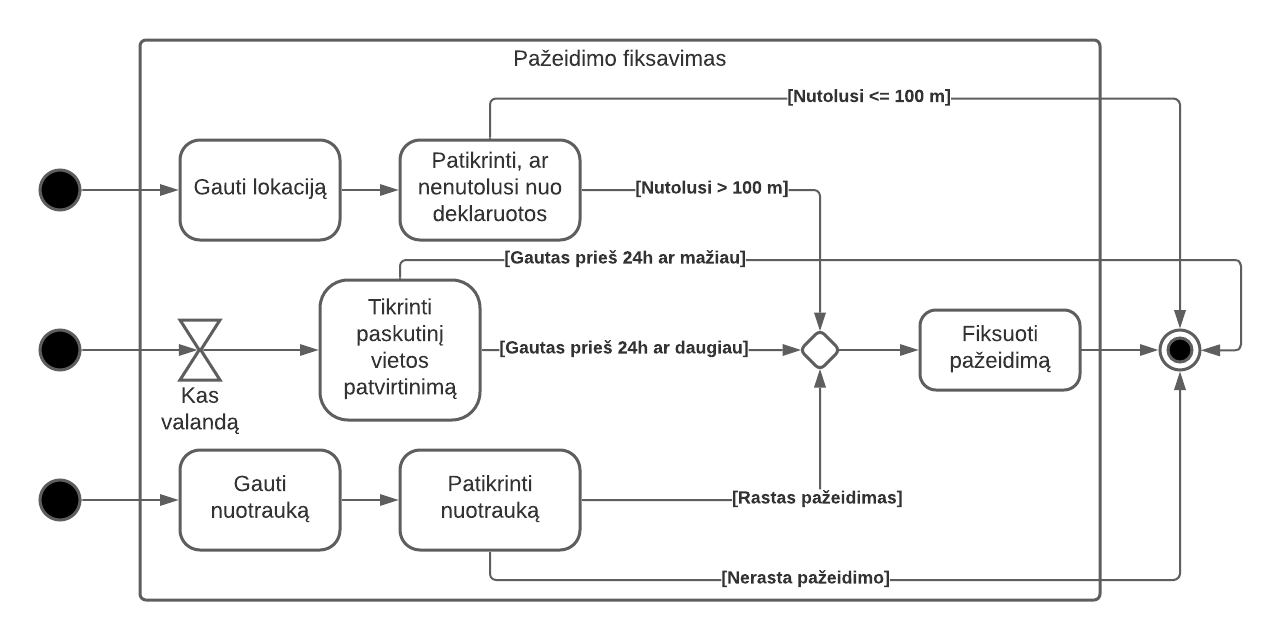
\includegraphics[scale=0.7]{img/business_process_identify_violation.png}
	\caption{Saviizoliacijos pažeidimo fiksavimo verslo procesas}
	\label{img:business_process_identify_violation}
\end{figure}

\subsection{Kaip?}\label{sec:vartotojoReqHow}
Šiame poskyriuje aprašomas projekto gylis - kokios transakcijos reikalingos (\ref{img:business_transactions} pav.), kokios verslo užduotys ir kiek yra kompiuterizuojamos. 

\subsubsection{Verslo transakcijos}
\begin{itemize}
	\item Būti įspėtam apie privalomą saviizoliaciją. Visos šią transakciją palaikančių procesų (saviizoliacijos ir jos pabaigos fiksavimo, pranešimo apie privalomą saviizoliaciją) užduotys yra vykdomos automatiškai.
	\item Patvirtinti saviizoliacijos laikymąsi. Visos šią transakciją palaikančio proceso „pranešimas apie privalomą saviizoliaciją" užduotys yra vykdomos automatiškai. Proceso „saviizoliacijos laikymosi patvirtinimas'' užduotis pateikti nuotrauką bei pateikti buvimo vietą yra kompiuterizuotos.
	\item Pranešti apie saviizoliacijos pažeidimą policijai. Visos šią transakciją palaikančių proceso „reikalingų duomenų perdavimas policijai" užduotys yra vykdomos automatiškai. Proceso visos „saviizoliacijos pažeidimo fiksavimas" užduotys yra vykdomos automatiškai, išskyrus patikrinti nuotrauką, kuri yra kompiuterizuota.
	\item Atnaujinti pavojingų šalių sąrašą. Šią transakciją palaikančio proceso „pavojingų šalių sąrašo atnaujinimas" užduotis yra kompiuterizuojama.
\end{itemize}

\begin{figure}[H]
	\centering
	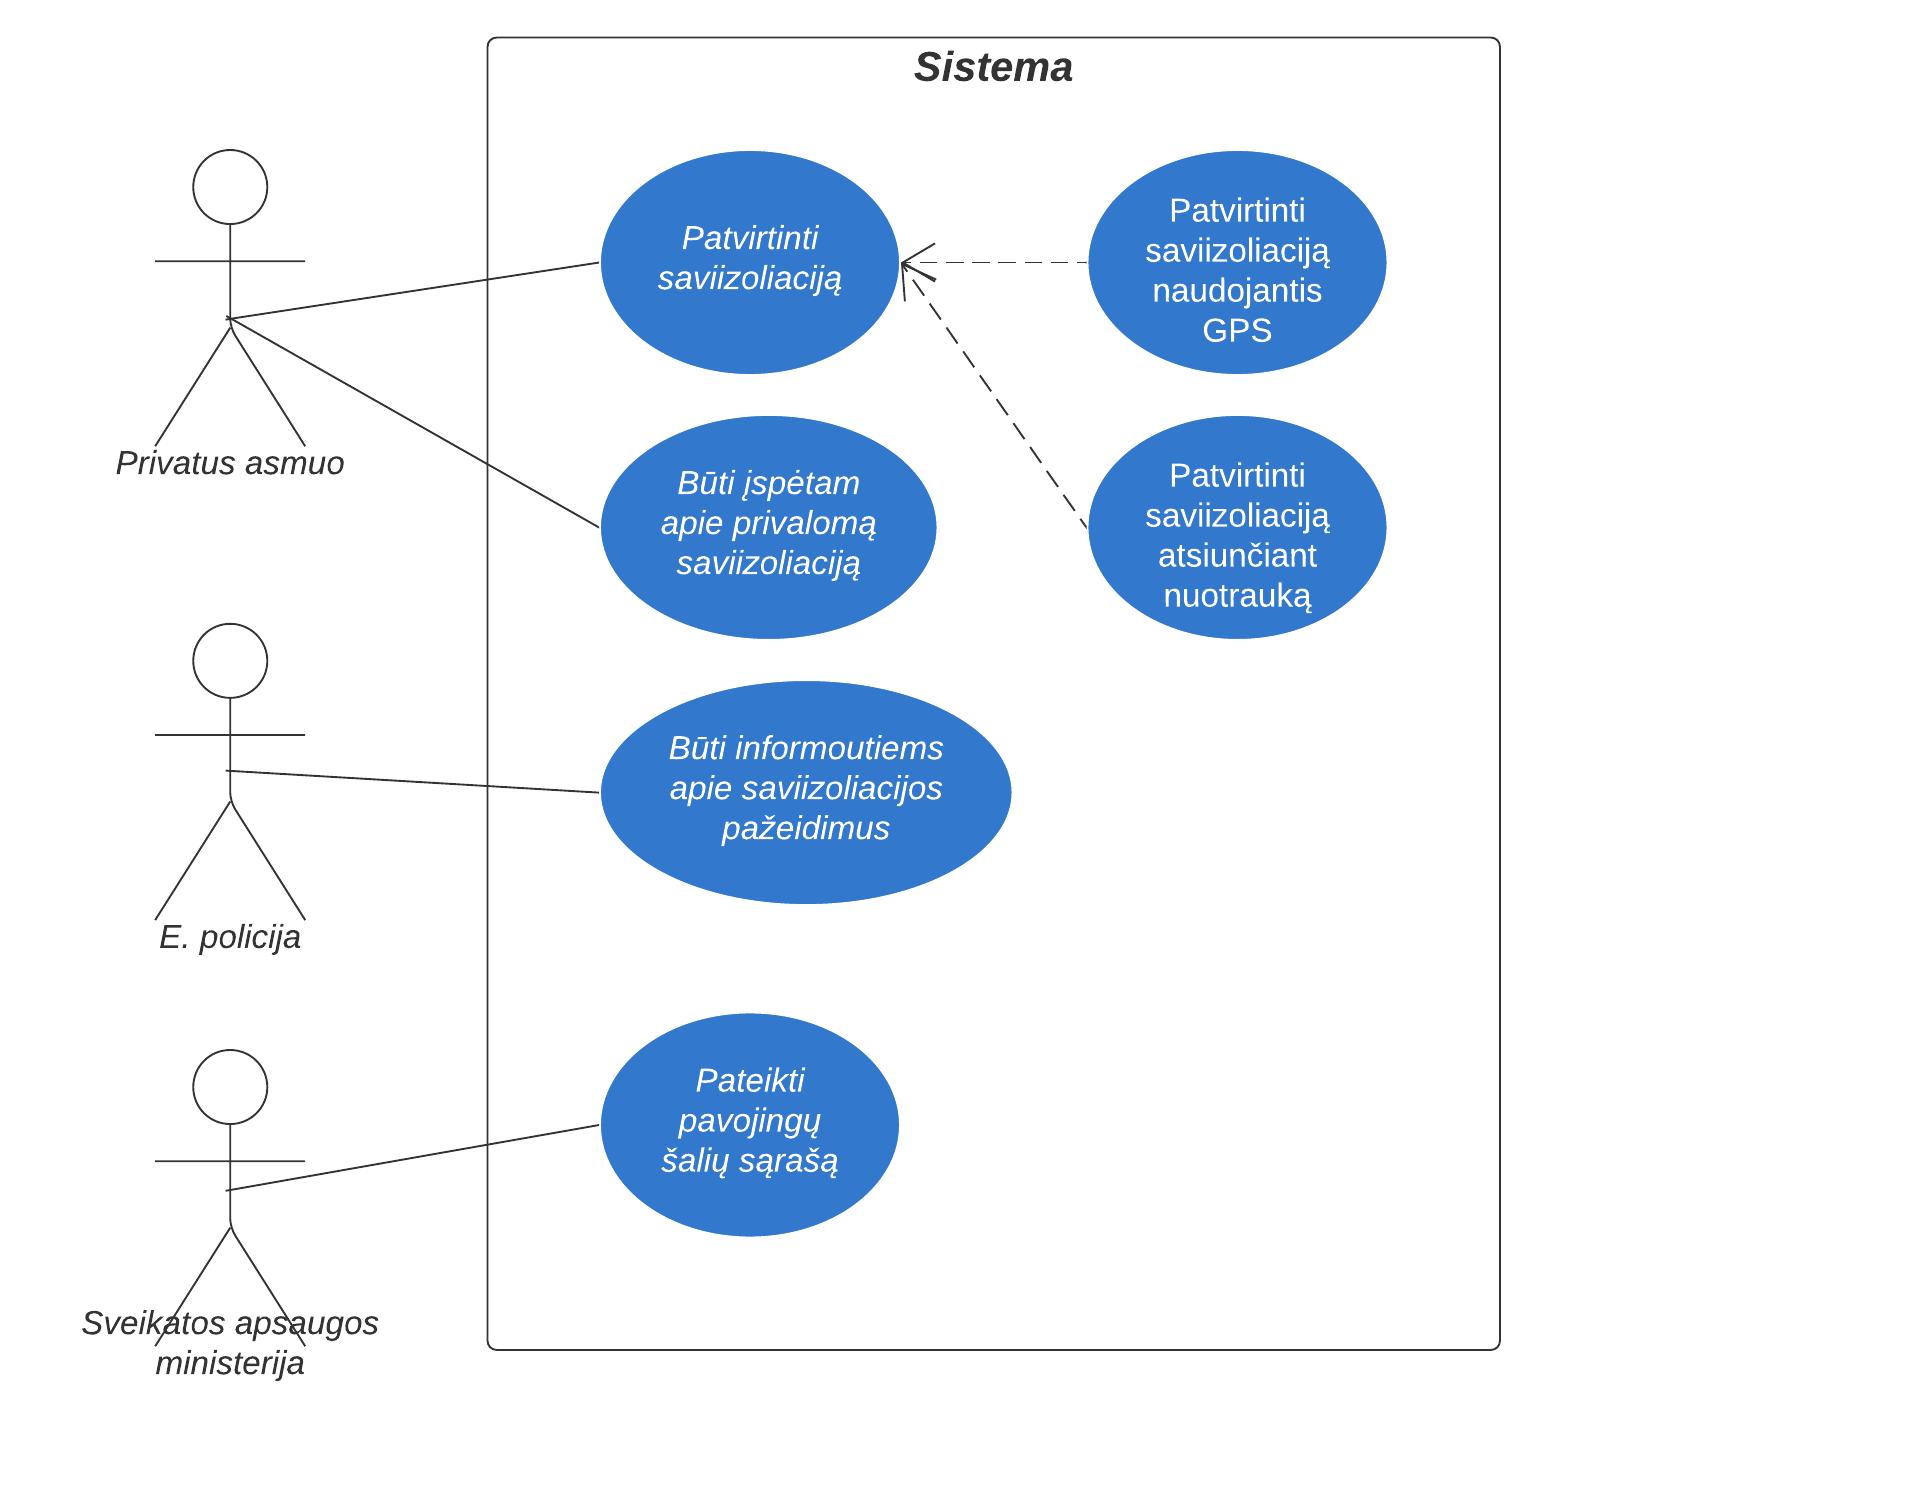
\includegraphics[scale=0.7]{img/use_case_diagram_user.png}
	\caption{Verslo transakcijos}
	\label{img:business_transactions}
\end{figure}

\subsubsection{Suvaržymai (nefunkciniai reikalavimai)}
Rezultatai, patikimumas bei saugumas yra labai svarbūs dėl informacijos kuria disponuojama jautrumo bei dalykinės srities rimtumo.

\textbf{Rezultatai}:
Turi būti teisingai identifikuojama 100\% privačių asmenų, kuriems reikalinga saviizoliacija ir tai galima nustayti pagal turimus duomenis. 
Turi būti teisingai nustatomi 99,9\% saviizoliacijos pažeidimų.

\textbf{Patikimumas}:
100\% asmenų turi būti informuojama apie privalomą saviizoliaciją. Apie 100\% pažeidimų turi būti informuojama e. policija.

\textbf{Saugumas}:
Saugumo reikalavimai turi būti aukšti. Projekte dirbama su asmenine žmonių informacija kuri gali būti susijusi su žmogaus sveikatos informacija. Sistema turi būti kiek galima saugesnė.

\subsection{Ką?}\label{sec:vartotojoReqWhat}
Šiame poskyriuje formuluojami verslo objektus modeliuojančių informacinių objektų reikalavimai.

\subsubsection{Informaciniai objektai}

Visiems aprašomiems informaciniams objektams (išskyrus šalis) taikomi aukščiausi saugumo reikalavimai, kadangi ši informacija yra jautri ir privati bei negali patekti tretiems asmenims.

\noindent\textbf{Privatus asmuo}:
\begin{itemize}
	\item Identifikatorius - asmens kodas.
	\item Baziniai rodikliai:
	\begin{itemize}
		\item Vardas - simbolių eilutė, leidžiami lietuviški bei lotyiniški simboliai bei tarpo simbolis. Privalomas.
		\item Pavardė - simbolių eilutė, leidžiami lietuviški bei lotyiniški simboliai bei tarpo simbolis. Privalomas.
		\item Telefono numeris - simbolių eilutė, atitinkanti formatą +3706*******, 86******* arba bet kokį telefono numeri su validžiu šalies kodu. Privalomas.
	\end{itemize}
\end{itemize}

\noindent\textbf{Saviizoliacija}:
\begin{itemize}
	\item Identifikatorius - unikalus sugeneruojamas kodas + saviizoliacijos pradžia. T. y. KKKKKKKYYMMDD, kur KKKKKKK - kodas, YY - du paskutiniai metų skaitmenys, MM - mėnuo, DD - diena.
	\item Baziniai rodikliai:
	\begin{itemize}
		\item Pradžia - data. Privalomas.
		\item Pabaiga - data. Neprivalomas.
		\item Priežastis - kelionė, kontaktas arba liga. Privalomas
		\item Saviizoliacijos vieta - adresas. Privalomas.
	\end{itemize}
	\item Sąryšiai:
	\begin{itemize}
		\item Privatus asmuo. Privalomas.
	\end{itemize}	
\end{itemize}

\noindent\textbf{Saviizoliacijos patvirtinimas}:
\begin{itemize}
	\item Identifikatorius - saviizoliacijos identifikatorius + data ir laikas. T. y. IDYYMMDDhhmmss, kur ID - saviizoliacijos identifikatorius, YY - du paskutiniai metų skaitmenys, MM - mėnuo, DD - diena, hh - valanda, mm - minutės, ss - sekundės.
	\item Baziniai rodikliai:
	\begin{itemize}
		\item Laikas - data ir laikas. Privalomas.
		\item Tipas - nuotrauka arba koordinatės. Privalomas.
		\item Vieta - koordinatės. Privalomas, jei tipas - koordinatės.
		\item Nuotrauka - adresas. Privalomas, jei tipas - nuotrauka.
	\end{itemize}
	\item Sąryšiai:
	\begin{itemize}
		\item Saviizioliacija. Privalomas.
	\end{itemize}	
\end{itemize}

\noindent\textbf{Saviizoliacijos pažeidimas}:
\begin{itemize}
	\item Identifikatorius - saviizoliacijos identifikatorius + data ir laikas, kuomet fiksuotas pažeidimas. T. y. IDYYMMDDhhmmss, kur ID - saviizoliacijos identifikatorius, YY - du paskutiniai metų skaitmenys, MM - mėnuo, DD - diena, hh - valanda, mm - minutės, ss - sekundės.
	\item Baziniai rodikliai:
	\begin{itemize}
		\item Laikas - data ir laikas. Privalomas.
		\item Tipas - nuotrauka, koordinatės arba jokio patvirtinimo. Privalomas.
		\item Vieta - koordinatės. Privalomas, jei tipas - koordinatės.
		\item Nuotrauka - adresas. Privalomas, jei tipas - nuotrauka.
	\end{itemize}
	\item Sąryšiai:
	\begin{itemize}
		\item Saviizioliacija. Privalomas.
	\end{itemize}	
\end{itemize}

\noindent\textbf{Šalis}:
\begin{itemize}
	\item Identifikatorius - šalies kodas (pagal ISO).
	\item Baziniai rodikliai:
	\begin{itemize}
		\item Pavadinimas - simbolių eilutė, leidžiami lietuviški ir lotyniški simboliai, tarpo, brūkšnio simboliai.
		\item Pradžia - data. Privalomas.
		\item Pavojinga - taip arba ne. Privalomas.
	\end{itemize}
\end{itemize}

\noindent\textbf{Atvykimas}:
\begin{itemize}
	\item Identifikatorius - unikalus vidinis identifikatorius.
	\item Baziniai rodikliai:
	\begin{itemize}
		\item Laikas - data ir laikas. Privalomas.
	\end{itemize}
	\item Sąryšiai:
	\begin{itemize}
		\item Šalis. Privalomas.
		\item Privatus asmuo. Privalomas.
	\end{itemize}	
\end{itemize}

\noindent\textbf{Ligos atvejis (susirgimas)}:
\begin{itemize}
	\item Identifikatorius - unikalus vidinis identifikatorius.
	\item Baziniai rodikliai:
	\begin{itemize}
		\item Laikas - data ir laikas. Privalomas.
	\end{itemize}
	\item Sąryšiai:
	\begin{itemize}
		\item Privatus asmuo. Privalomas.
		\item Kontaktai. Privalomas (0 - *).
	\end{itemize}	
\end{itemize}

\noindent\textbf{Kontaktas}:
\begin{itemize}
	\item Identifikatorius - unikalus vidinis identifikatorius.
	\item Baziniai rodikliai:
	\begin{itemize}
		\item Laikas - data ir laikas. Privalomas.
		\item Vieta - koordinatės. Neprivalomas.
	\end{itemize}
	\item Sąryšiai:
	\begin{itemize}
		\item Privatus asmuo. Privalomas.
		\item Privatus asmuo. Privalomas.
	\end{itemize}	
\end{itemize}

\noindent\textbf{Testo rezultatas}:
\begin{itemize}
	\item Identifikatorius - unikalus vidinis identifikatorius.
	\item Baziniai rodikliai:
	\begin{itemize}
		\item Laikas - data ir laikas. Privalomas.
		\item Rezultatas - teigiamas arba neigiamas. Privalomas.
	\end{itemize}
	\item Sąryšiai:
	\begin{itemize}
		\item Privatus asmuo. Privalomas.
	\end{itemize}	
\end{itemize}

\noindent\textbf{Pranešimas apie privalomą saviizoliaciją}:
\begin{itemize}
	\item Identifikatorius - unikalus vidinis identifikatorius.
	\item Baziniai rodikliai:
	\begin{itemize}
		\item Laikas - data ir laikas. Privalomas.
		\item Tekstas - simbolių eilutė, leidžiami lietuviški ir lotyniški simboliai, tarpo ir skyrybos ženklai. Privalomas.
	\end{itemize}
	\item Sąryšiai:
	\begin{itemize}
		\item Privatus asmuo. Privalomas.
	\end{itemize}	
\end{itemize}

\subsubsection{Kalendoriniai ir verslo įvykiai}

\begin{itemize}
	\item Gauta informacija (pateikta muitinės) apie atvykusį iš pavojingos šalies privatų asmenį.
	\item Gauta informacija apie susirgimą (teigiamą testą).
	\item Gauta informacija apie pasveikimą (pakartotinį neigiamą testą).
	\item Gauta informacija apie neigiamą testą.
	\item 2 savaitės po saviizoliacijos pradžios (saviizoliacijos pabaigai identifikuoti).
	\item Privalomos saviizoliacijos fiksavimas.
	\item SAM naujo pavojingų šalių sąrašo paskelbimas.
	\item Kas 12 valandų nuo saviizoliacijos pradžios (priminimui apie saviizoliacijos patvirtinimą).
	\item Privataus asmens buvimo vietos arba nuotraukos pateikimas.
	\item Kiekvieną valandą (saviizoliacijos duomenų nepateikimui identifikuoti).
	\item Pažeidimo užfiksavimas.
\end{itemize}

\subsection{Kas?}\label{sec:vartotojoReqWho}

Šiame poskyriuje detalizuojami, konkretizuojami ir tikslinami vykdytojų reikalavimai, suformuluoti formuluojant verslo reikalavimus. Naudotojai:
\begin{center}
	\setstretch{1.0}
	\small
	\begin{longtable}{|L{2cm}|C{3cm}|C{3cm}|C{3cm}|C{3cm}|}
		\caption{IS naudotojai}
		\label{table:users}
		\\ \hline
		Naudotojas & Prieigos teisės & Įgaliojimai & Kompetencijos & Panaudojamumas \\ \hline
		Privatus asmuo & Gauti įspėjimą apie privalomą saviizoliacijos laikymąsi - peržiūrėti sau adresuotą \emph{pranešimą apie privalomą saviizoliaciją} SMS žinutėje; & Saviizoliacijos metu privalo pateikti ir patvirtinti savo geografines koordinates, siųsti saviizoliaciją patvirtinančią nuotrauką - kurti savo \emph{saviizoliacijos patvirtinimus} per visuomenei skirtą svetainę. & Baziniai kompiuterinio raštingumo įgūdžiai, užtenka pagrindinėje mokykloje dėstomo informatikos kurso. & Naudojasi tik tada, kai būna saviizioliacijoje, du kartus per parą po kelias minutes. Turi būti sudarytos galimybės naudotis neįgaliesiems. \\ \hline
		Sveikatos apsaugos ministerija & Pateikti pavojingų šalių sąrašą - peržiūrėti, redaguoti, pridėti bei trinti \emph{šalis} per epidemiologams skirtą internetinę svetainę. & Privalo patvirtinti, jog pateiktas šalių sąrašas yra korektiškas; & Baziniai kompiuterinio raštingumo įgūdžiai, užtenka pagrindinėje mokykloje dėstomo informatikos kurso. & Naudojasi daugiausia kartą per dieną, iki 30 minučių. \\ \hline
		Muitinė & Pateikti iš pavojingų šalių atvykusių žmonių sąrašą - kurti \emph{atvykimo} informacinius objektus. Tamp naudojama programinė sąsaja. & Privalo patvirtinti, jog pateikiamas žmonių sąrašas yra korektiškas & Nėra (procesas pilnai automatizuotas) & Nėra (procesas pilnai automatizuotas)                                     \\ \hline
	\end{longtable}
\end{center}

\subsection{Kur?}\label{sec:vartotojoReqWhere}
Šiame poskyriuje detalizuojama, kokie prieigos prie sistemos mazgai už kokį panaudos atvejį yra atsakingi bei kur yra saugomi informaciniai objektai.

\begin{itemize}
	\item Saviizoliacijos patvirtinimas - visuomenei skirtoje internetinėje svetainėje. Duomenys apie patvirtinimą saugomi sistemoje 14 kalendorinių dienų.
	\item Būti įspėtam apie privalomą saviizoliaciją - SMS žinute. Įspėjimai sistemoje nesaugomi.
	\item Pateikti pavojingų šalių sąrašą - epidemiologams skirtoje internetinėje svetainėje. Šalių sąrašas saugomas sistemoje.
\end{itemize}

\subsection{Kada?}\label{sec:vartotojoReqWhen}

Šiame poskyriuje nurodomi laiko suvaržymai verslo panaudos atvejams.

\begin{itemize}
	\item Saviizoliacijos patvirtinimas - vidutiniškai turėtų trukti 2 minutes.
	\item Būti įspėtam apie privalomą saviizoliaciją - vidutiniškai iki 1 valandos po informacijos apie pavojų gavimo.
	\item Pateikti pavojingų šalių sąrašą - maksimali trukmė - 15 minučių.
\end{itemize}

\section{IS reikalavimai}

\subsection{Kodėl?}\label{sec:ISReqWhy}
Suformulavus ir išanalizavus vartotojų reikalavimus, buvo suformuluota šitokia naujos viruso valdymo informacinės sistemos vizija:
Produktas „Saviizoliacijos užtikrinimo informacinė sistema“ skirtas infekcinių ligų centrams, kuriems reikia tvarkyti visą informaciją susijusią su 
žmonėmis užsikrėtusiais virusine ligą, jiems reikalingą arba nereikalingą izoliaciją bei sekti kaip žmonės laikosi saviizoliacijos.
Tai kompiuterizuota sistema, kuri automatizuotai tvarko informaciją apie susirgusius virusu žmones, praneša virusu užsikrėtusiui žmogui bei kontaktiniams asmenims 
trumpąją žinutę apie turėtą kontaktą bei praneša policijai apie saviizoliacijos pažeidimus. Skirtingai nei senoji informacinė sistema, informacija yra tvarkoma
automatizuotai, pasitelkiama kompiuterinė skaičiuojamoji galia, žmonių informacimas trunka vos kelias sekundes, o policija pranešimus apie saviizoliacija gauna centralizuotai.
Tai keičia visa viruso valdymo sistemą: informacija yra vienoje sistemoje, ji pasiekiama centralizuotai ir po to gali būti išskirstyta į kitas sistemas.
Sistema leis užtikrinti, kad duomenys būtų prieinamami tik tiems žmonėms, kurie turi teises prie žmogaus asmens duomenų, kas nebuvo užtikrinama iki dabar.
\medskip
Funkcinių galimybių medis:

\begin{enumerate}
\item Galimybė tvarkyti visą su saviizoliacija susijusią informaciją.
	\begin{enumerate}
		\item Galimybė tvarkyti saviizoliacijos asmenų registrą.
		\begin{enumerate}
			\item Galimybė fiksuoti užsikrėtujusio saviizoliaciją.
			\item Galimybė fiksuoti užsikrėtujusio kontaktus. Užsikrėtujusių kontaktų izoliacija fiksuojama automatiškai.
			\item Galimybė fiksuoti pasveikusio saviizoliacijos pabaigą.
			\item Galimybė fiksuoti saviizoliacijos pabaigą, kai ši trunką ilgiau nei dvi savaites.
		\end{enumerate}
		\item Galimybė pranešti užsikrėtusiąjam apie saviizoliacijos pradžią SMS žinute.
		\item Galimybė atnaujinti pavojingų šalių sąrašą.
	\end{enumerate}
	\item Galimybė tvarkyti visą su saviizoliacijos užtikrinimu susijusią informaciją.
	\begin{enumerate}
		\item Galimybė siųsti patvirtinimo prašymą saviizoliuojančiam asmeniui.
		\item Galimybė gauti saviizoliacijos patvirtinimą iš saviizoliuojančio asmens.
		\item Galimybė fiksuoti saviizoliacijos pažeidimą.
	\end{enumerate}
	\item Galimybė tvarkyti visą su saviizoliacijos pažeidimais susijusią informaciją.
	\begin{enumerate}
		\item Galimybė pranešti apie saviizoliacijos pažeidimą policijai.
	\end{enumerate}
\end{enumerate}

Medį papildo tokios viruso valdymo informacinės sistemos taisyklės:
\begin{enumerate}
	\item Žmogus į saviizoliacijos registrą gali būti įtrauktas tik vieną kartą, jo identifikatorius turi būti asmens kodas. Jeigu asmens kodas keičiasi, asmuo gali būti įtrauktas ir antrą kartą.
	\item Žmogaus saviizoliacija yra automatiškai baigiama po 2 savaičių nuo jo įrašymo saviizoliacijos asmenų registre.
	\item Sistemoje turi būti užtikrinama, jog žinutę dėl saviizoliacijos gaus tik reikiami žmonės ir nebus sukeliama panikos kitiems žmonėms.
	\item Informacija policijai yra perduodama automatiškai per elektroninį laišką. Turi būti saugoma žymą, kada policija patvirtino, jog gavo laišką.
\end{enumerate}

Verslo sistemos analizės metu išryškintos šios verslo problemos:
\begin{enumerate}
	\item Žmonės nežino kada jiems reikalinga izoliacija, kai sužinoma, dažniausiai būna praėjęs ilgas laiko tarpas.
	\item Policija nespėja reaguoti į saviizoliacijos pažeidimus bei tikrinti kiekvieno besiizoliuojančio asmens.
	\item Visi duomenys susije su viruso valdymų yra "išmėtyti" po skirtingas sistemas ir nėra niekur centralizuojami.
\end{enumerate}

Visų tų problemų priežastis yra prasta viruso pandemijos valdymo informacinė sistema.

\subsection{Kaip?}\label{sec:ISReqHow}

Sistemos funkciniai komponentai:
\begin{enumerate}
	\item Izoliuotų asmenų registras.
	\begin{enumerate}
		\item Galimybė fiksuoti užsikrėtujusio saviizoliaciją.
		\item Galimybė fiksuoti užsikrėtujusio kontaktus. Užsikrėtujusių kontaktų izoliacija fiksuojama automatiškai.
		\item Galimybė fiksuoti pasveikusio saviizoliacijos pabaigą.
		\item Galimybė fiksuoti saviizoliacijos pabaigą, kai ši trunką ilgiau nei dvi savaites.
	\end{enumerate}

	\item Pavojingų šalių registras.
	\begin{enumerate}
		\item Galimybė atnaujinti pavojingų šalių sąrašą.
	\end{enumerate}

	\item Saviizoliacijos pranešimų sistema.
	\begin{enumerate}
		\item Galimybė pranešti užsikrėtusiąjam apie saviizoliacijos pradžią SMS žinute.
 		\item Galimybė pranešti apie saviizoliacijos pažeidimą policijai.
	\end{enumerate}

	\item Savitarnos portalas žmonėms, kur suteikiama informacija apie izoliaciją bei kita svarbi informacija.
	\begin{enumerate}
		\item Galimybė siųsti patvirtinimo prašymą saviizoliuojančiam asmeniui.
		\item Galimybė gauti saviizoliacijos patvirtinimą iš saviizoliuojančio asmens.
		\item Galimybė fiksuoti saviizoliacijos pažeidimą.
	\end{enumerate} 

	\item Mobilioji programėle skirta patvirtinti saviizoliaciją ir sekti saviizoliuojančio žmogaus GPS vietą.
	\begin{enumerate}
		\item Galimybė siųsti patvirtinimo prašymą saviizoliuojančiam asmeniui.
		\item Galimybė gauti saviizoliacijos patvirtinimą iš saviizoliuojančio asmens.
		\item Galimybė fiksuoti saviizoliacijos pažeidimą.
	\end{enumerate} 

\end{enumerate}

\textbf{Rezultatai}:
Turi būti teisingai identifikuojama 100\% privačių asmenų, kuriems reikalinga saviizoliacija ir tai galima nustayti pagal turimus duomenis. 
Turi būti teisingai nustatomi 99,9\% saviizoliacijos pažeidimų.

\textbf{Patikimumas}:
100\% asmenų turi būti informuojama apie privalomą saviizoliaciją. Apie 100\% pažeidimų turi būti informuojama e. policija.

\textbf{Saugumas}:
Saugumo reikalavimai turi būti aukšti. Projekte dirbama su asmenine žmonių informacija kuri gali būti susijusi su žmogaus sveikatos informacija. Sistema turi būti kiek galima saugesnė.

\subsection{Ką?}\label{sec:ISReqWhat}
Saviizoliacijos užtikrinimo naujoje informacinėje sistemoje turėtų būti numatytos šios informacijos saugyklos:
\begin{enumerate}
	\item Izoliuotų asmenų duomenų bazę. 
	Tai yra izoliuotų asmenų duomenų bazė kurioje saugomi duomenyts apie izoliuotus asmenis. Rašyti naujus įrašus į duomenų bazę gali 
	tik epidemiologai arba jie automatiškai importuoji iš e - sveikatos sistemos. Įrašai pateikiami darbuotojo darbo vietos kompiuterio ekrane. 
	Į bazę galima rašyti tik įrašus, kuriuose visi laukai yra užpildyti. Už įraše pateiktos informacijos korektiškumą atsako tą įrašą sukūręs darbuotojas.

	\item Paveiktų šalių duomenų bazę.
	Tai šalių duomenų bazė, kurioje nurodytas šalies paveikimo lygis. Šią informaciją gali keisti tik ministras arba ministro įgalioti 
	asmenys. Duomenys yra pasiekiami visiems sistemos naudotojams ir išorės žmonėms. 
	Įrašai pateikiami darbuotojo darbo vietos kompiuterio ekrane.
	Į bazę galima rašyti tik įrašus, kuriuose visi laukai yra užpildyti.
	Už įraše pateiktos informacijos korektiškumą atsako tą įrašą sukūręs darbuotojas.

	\item Saviizoliacijos patvirtinimo duomenų bazę.
	Tai saviizoliacijos patvirtinimų duomenų bazė. Įrašai pateikiami iš izoliuojančio asmens mobiliajame telefone esančios programėlės.
	Į bazę galima rašyti tik įrašus, kuriuose visi laukai yra užpildyti.
	Už įraše pateiktos informacijos korektiškumą atsako tą įrašą sukūręs asmuo.

	\item Išsiųstų pranešimų duomenų bazė.
	Įrašai automatiškai įrašomi į pranešimų duomenų bazę, kai bet koks pranešimas žmogui apie būtina izoliaciją, apie kontakto turėjimą yra išsiunčiamas. 

	\item Pažeidimų duomenų bazė. 
	Įrašas įvedamas į duomenų bazę, kai pažeidimas yra užfiksuotas. 
	Į bazę galima rašyti tik įrašus, kuriuose visi laukai yra užpildyti.
	Už įraše pateiktos informacijos korektiškumą atsako tą įrašą sukūręs darbuotojas.
\end{enumerate} 

\subsection{Kas?}\label{sec:ISReqWho}

Sistema turi būti lengvai atpažįstama, lengvai išmokstama ir nesunkiai naudojama.
Sistema bus galima naudotis per kelis interfeisus:
\begin{enumerate}
	\item Savitarnos puslapį.
	\item Mobiliąją programėlę.
\end{enumerate} 

Bendravimas su interfeisais vyks per interneto naršyklę HTTPS protokolu. Prieigos teisės plačiau aprašytos skyrelyje "Vartotojo reikalavimai - kas?"

\subsection{Kur?}\label{sec:ISReqWhere}

Sistema bus kuriama pasinaudojant Amazon Web Services teikiamomis paslaugomis. 
Kad vartotojas pasinaudotų sistema, darbo vietoje turi būti įdiegta bet kokia naujos kartos naršyklė (Edge, Firefox, Chrome) bei operacinė sistema (LINUX, Mac OS, Windows 7, Windows XP, Windows 10, Windows X)
Naudotis sistema nereikalingi jokie išskirtiniai įrangos našumo reikalavimai.
Kad vartotojas pasinaudotų mobiliąja programėle, jo telefone turi būti įrašyta Android arba iOS operacinė sistema ir programėlė turi būti parsisiųsta iš autoretetingo šaltinio: Play Store arba App Store.
\subsection{Kada?}\label{sec:ISReqWhen}

Laiko reikalavimai:
\begin{itemize}
	\item Prisijungimas prie sistemos turi trukti iki minutės
	\item Pateikimas apie saviizoliacijos laikymąsi turi trukti iki minutės
	\item Saviizoliacijos patvirtinimas - vidutiniškai turėtų trukti 30 sekundžių.
	\item Būti įspėtam apie privalomą saviizoliaciją - iki vienos minutės po informacijos apie pavojų gavimo.
	\item Pateikti pavojingų šalių sąrašą - maksimali trukmė - 1 minutė.
\end{itemize}

\section{PS reikalavimai}
 
\subsection{Kodėl?}\label{sec:PSReqWhy}
Šiame skyriuje formuluojami programų sistemos specifikacijos vizija bei realizacijos apribojimai

\textbf{Vizija:} Vizija sutampa su produkto vizija - centralizuota viruso valdymo sistema infekcinių ligų centrams, kuri automatiškai tvarko informaciją apie virusu susirgusius žmones, informuoja užsikrėtusius ir kontaktinius asmenis apie turėtą kontaktą bei praneša policijai saviizoliacijos pažeidimo atvejį.z

\textbf{Ekonominiai apribojimai:}
Sistema bus apribojama šiais ekonominiais aspektais:
	\begin{enumerate}
		\item Programų sistemos kūrimo kaštai - reikiamų specialistų (programuotojų, vartotojų potyrio specialistų, verslo analitikų, testuotojų) samdymas programų sistemos kūrimo laikotarpiui, reikiamų įrankių licenzijų įsigijimo kainos, įrangos, reikalingos programų sistemos kūrimui, kainos ir t.t. 
		\item Programų sistemos diegimo kaštai - kadangi programų sistema bus internetinė svetainė, numatyta programų sistemą į debesį, o sistemą pasieks konkrečius įrengtus terminalus.
		\item Palaikymo kainos - reikiamų specialistų (programuotojo, testuotojo ir kitų specialistų) samdymas programų sistemos palaikymo laikotarpiui, reikiamų įrankių licenzijų įsigijimo kainos, įrangos, reikalingos programų sistemos palaikymui, kainos ir t.t.
		\item Kadangi sistema skirta sekti epidemiologijos situacija šalyje - sistemą bus galima pernaudoti skirtingoms epidemiologijoms, tačiau negalima pernaudoti skirtingoms šalims, nes gaunami duomenys priklauso nuo išorinių sistemų, o informaciniais objektai šalyse gali irgi skirtis 
	\end{enumerate}

\textbf{Politiniai apribojimai:} Laikantis organizacijos politikos - organizacijos darbuotojai, dirbantys su sistema: ar tai dirbantys prie sistemos kūrimo, testavimo, palaikymo ir t.t., privalo laikytis konfidencialumo sutartyje nurodytų įsipareigojimų.

\textbf{Teisiniai apribojimai:} sistema laikysis Lietuvos Respublikos ir Europos Sąjungos teisinių apribojimų.

\subsection{Kaip?}\label{sec:PSReqHow}
	\subsubsection{Programų sistemos tinkamumo reikalavimia}
		\subsubsubsection{Galimybė valdyti užsikėtusių žmogaus duomenis}
			Pradiniai duomenys - žmogaus asmeniniai duomenys, kontaktiniai duomenys, saviizoliacijos pradžios ir numatomos pabaigos data, sarašas su kuo kontaktavo susirgęs žmogus.
			\\
			Gautas rezultatas - įvesti žmogaus saviizoliacijos duomenis į registrą, galimybė tos duomenis perduoti kitoms posistemėms.
		\subsubsubsection{Galimybė valdyti pavojingų šalių registrą}
			Pradiniai duomenys - nauja informaciją apie pavojingas šalis
			\\
			Gautas rezultatas - atnaujintas pavojingų šalių sąrašas kurį naudos kitos posistemės.
		\subsubsubsection{Galimybė valdyti sviizoliacijos pranešimų sistema}
			Pradiniai duomenys - užsikrėtusių žmonių registro duomenys, žmogaus lokacijos duomenys
			\\
			Gautas rezultatas - žmogus informuotas apie jam paskitrą saviizoliacijos laikotarpį SMS žinute. Policija informuojama žmogui pažeidus saviizoliaciją.
		\subsubsubsection{Galimybė valdyti portalo apie saviizoliacijos informaciją}
			Pradiniai duomenys - užsikrėtusiųjų registras, žmogaus lokacijos duomenys
			\\
			Gautas rezultatas - gauti ir atvaizduojama žmogaus saviizoliacijos būsena.
		\subsubsubsection{Galimybė valdyti mobilioji aplikaciją saviizoliacijai sekti}
			Pradiniai duomenys - žmogaus GPS lokacija, užsikėtusiųjų registras
			\\
			Gautas rezultatas - įsitikint, kad žmogus nepažeidžia saviizoliacijos reikalavimų.
	\subsubsection{Programų sistemos sąveikos su kitomis sistemomis}
		Sistema sąveikaus su: e. policijos sistema, NVSC sistema, sveikatos ministerijos sistema, muitinės sistema, e. sveikatos sistema, karštosios linijos sistema, renginų organizatorių sistema.
	\subsubsection{Programų sistemos atitikimas galiojantiems teisės aktams}
		Sistema atitinka Lietuvos ir Europos teisės aktams. 
		Sistema taip pat laikosi BDAR reglamento.
	\subsubsection{Programų sistemos trasuojamumo reikalavimai}
		Sistemos atrasuojamumas bus įgyvendinatas pasinaudojant Jira Atlassian sistema kuri užtikrina programos trsuojamumą
	\subsubsection{Programų sistemos patikimumo reikalavimai}
		Sistema turi išlikti pasiekiama 99 procentus laiko.
		Įvykus sistemos tiktims sistema turi sugebėti automatiškai pasileisti išnaujo neprarasdama duomenų.
	\subsubsection{Programų sistemos išbaigtumas}
		Užsakovui priimtimas vienas tikdis per dieną.
		Trumpiausias laikas tarp dviejų trikdžių yra 24 valandos.
		Sistemoje neturi būti palikta esminių klaidų.
	\subsubsection{Programų sistemos atsparumo triktims reikalavimai}
		Dėl trikdžiū sistema gali neveikti 1 valandą per diena.
		Sistemoje gali būti vienas įsilaužimas per mėsenį.
	\subsubsection{Programų sistemos atkuriamumo reikalavimai}
		Sistema turi galėti atsikurti per valandą po sutrikimo.
		Per valandą turi būti atkūriami prarasti duomenys ir funkcionalumas.
		Trikdis turi būti rastas ir pašalintas per savaitę.
		
	\subsubsection{Programų sistemos prieinamumo reikalavimai}
		Per dieną sistema turi išlikti funkcionali 23 valandas. 
	\subsubsection{Programų sistemos pažeidžiamumo reikalavimai}
		Esminis sistemos funkcionalumas turi būti atkurtas per valandą.
	\subsubsection{Programų sistemos aptarnavimo reikalavimai}
		Sistema turi būti galima atstatyi per valandą.
		Surastas trigdis programiniam kode turi būti pašalintas per savaitę.
	\subsubsection{Programų sistemos diegimo reikalavimai}
		Sistema yra paleidžiama debesų kompiuterijos srveriuose, todėl sistemos diegimo kaštai yra minimlūs.
		Sistemai perkelti iš vieno debesijos serverio į kitą turi pakakti 24 valandų darbo.
		Sistema perkeliama perkelus sukompiliuotus binarinius failus.
	\subsubsection{Programų sistemos adaptuojamumo reikalavimai}
		Perkelti sistema ant naujos platformos kainuotų 10000 žmogaus darbo valandų.
		\\
		Perkelti sistemą į kitą kompiuterinę platformą 20 žmogaus darbo valandų
		\\ 
		Perkelti sistemą į naujasnę operacinės sistemos versiją kainuotų 100 žmogaus darbo valandų
		\\
		Perkelti sistemos duomenis į nauja DBVS kainuotų 200 žmogaus darbo valandų.
	\subsubsection{Programų sistemos instaliuojamumo reikalavimai}
	\subsubsection{Programų sistemos atitikimo keliamumo standartams reikalavimai apibūdina}
	\subsubsection{Programų sistemos pakeičiamumo reikalavimai}
	\subsubsection{Programų sistemos prižiūrimumo reikalavimai}
	\subsubsection{Programų sistemos analizuojamumo reikalavimai}
	\subsubsection{Programų sistemos keičiamumo reikalavimai}
	\subsubsection{Programų sistemos stabilumo reikalavimai}
	\subsubsection{Programų sistemos testuojamumo reikalavimai}
	\subsubsection{Programų sistemos tvarkomumo reikalavimai}
	\subsubsection{Programų sistemos pakartotino panaudojamumo reikalavimai}

\subsection{Ką?}\label{sec:PSReqWhat}
Programų sistema digitalizuotus informacijos objektus saugos duomenų bazėse, kuriuose duomenys bus užšifruoti. Duomenų saugojimas atitiks numatytą duomenų apsaugos reglamentavimą pagal BDAR. Duomenys bus apsaugojami nuo tyčinių ir netyčinių grėsmių (pvz., duomenų pasiekimas neautorizuotiems asmenims).

\textbf{Programų sistemos duomenų apsaugos reikalavimai:}
\begin{itemize}
	\item Atsiradus atvejui, kad duomenys yra prarandami arba sugadinami, bus naudojama duomenų atstatymo procedūros, pvz. duomenų saugyklos versijų kontrolės versijos atkūrimas.
	\item Atsiradus atvejui, kad duomenys bus tyčia prarandami/gadinami arba neautorizuotai pasiekti, bus vykdomos organizacijos politikos procedūros - tikrinami konfidencialumo sutarties pažeidimai, apie atsiradusį atvejai pranešama policijai ir kt.
	\item Neautorizuotiems naudotojams nebus vaizduojama konfidencialūs duomenys, pvz., asmens kodas, siekiant užtikrinti duomenų apsaugos reglamentavimą pagal BDAR.
	\item Vaizduojant digitalizuotus informacijos objektus, nebus vaizduojami unikalūs vidiniais identifikatoriai.
\end{itemize}

\subsection{Kas?}\label{sec:PSReqWho}
\subsection{Kur?}\label{sec:PSReqWhere}
\subsection{Kada?}\label{sec:PSReqWhen}

\newpage

\sectionnonum{Rezultatai ir išvados}
Darbe suformuluoti sistemos, skirtos sekti epidemiologinę situaciją šalyje, 
reikalavimai: naudojantis Zachmano karkasu identifikuoti verslo, vartotojo,
informacinės sistemos bei programinės įrangos reikalavimai. Identifikavus norimas
sistemos savybes galima daryti išvadą, jog sistema išties palengvintų epidemiologinės
situacijos valdymą. Negana to, stebint dabartinę situaciją, galima teigti, jog sistemos 
aktualumas artimiausiu metu tik augs.

\newpage

\sectionnonum{Sąvokos}

\noindent\textbf{Epidemiologija} -- tai mokslas apie su sveikata susijusių įvykių (dažniausiai – sveikatos sutrikimų, ligų ar mirčių, bendrai vadinamų baigtimis) ir juos lemiančių veiksnių (vadinamų rizikos veiksniais) atsiradimą ir plitimą tam tikroje populiacijoje bei apie profilaktikos priemonių taikymo galimybes ir veiksmingumą. \\
\noindent\textbf{E. policija} -- policijos e-paslaugų portalas. \\
\noindent\textbf{Kontaktas} -- kontaktas veidas į veidą ne didesniu kaip dviejų metrų atstumu ilgiau nei 15 minučių. \\
\noindent\textbf{Pavojinga šalis} -- SAM įvardinta šalis, kurioje šiuo metu yra prasta epidemiologinė situacija ir iš kurios atvykstant reikia saviizoliuotis. \\
\noindent\textbf{Saviizoliacija} --karantinasm, apsiribojimas nuo visų socialinių kontaktų ir buvimas tik namuose. \\
\noindent\textbf{Sveikatos apsaugos ministerija (SAM)} -– Lietuvos Vyriausybės pagrindinė institucija, atsakinga už Lietuvos nacionalinės sveikatos politikos įgyvendinimą ir koordinavimą. \\
\noindent\textbf{SMS žinutė} -- trumpoji žinutė, daugelyje mobiliųjų telefonų esanti paslauga, skirta trumpųjų žinučių siuntimui tarp mobiliųjų telefonų arba kitų panašių įrenginių. \\

\end{document}



